\chapter{波动方程（补充）}
\label{chap:wave-equations}

拨动一根绷紧的弦然后松手。指尖离开的瞬间弦是一条折线，速度处处为零；片刻之后折角分成两个，各自向两端跑去，碰到琴桥又翻转回来。如果换成用小锤敲击，弦的初始形状是平的，却有一段初速度，随后的运动又完全不同。第~\ref{chap:diffusion-equations}章的热传导只要知道初始温度，这里却要同时知道初始位移和初始速度，时间导数多了一阶，整个演化的性格就变了。

最直接的差别有三个。温度的鼓包会被抹平，再也回不到原样，弦上的波却带着折角一直走下去，没有衰减，也没有变光滑。热方程在正时刻处处感受到初值的变化，弦上的一点却要等波跑过来才知道远处发生了什么。扩散的平方范数单调减小，弦的动能和弹性能却彼此转换，总量不变。

本章把这几点讲清楚，作为椭圆和扩散两章之外的补充。先由弦的受力写出方程，比较各种端点条件。一维实轴上的解可以完全写出来，它把初始数据分成左右两列行波，并告诉我们每个时空点依赖哪段初值。端点的作用用反射解释，区间上的解用模式展开，边界条件决定可以用哪些模式。

外力和边界驱动的影响用脉冲叠加算出。最后两节离开具体公式：能量恒等式给出守恒和唯一性，局部能量估计说明扰动不会超出传播锥，这两个结论在高维同样成立。高维的波没有左右两列的分解，本章只讨论能在高维保留下来的结论，具体的高维解公式不作推导。

\section{波动问题}
\label{sec:wave-problem}

一根弦的运动由什么决定？先从受力写出方程，看清位移、速度、波速和外力各自的位置，再讨论弦的端点能怎样约束运动。

\paragraph{从张力到方程}
设弦静止时沿$x$轴拉直，线密度（单位长度的质量）为常数$\rho>0$，张力大小为常数$\kappa>0$。记$u(x,t)$为点$x$在时刻$t$的竖直位移。我们只考虑小振动：斜率满足$\lvert\partial_xu\rvert\ll1$，弦上各点只沿竖直方向运动。

取一小段$[x,x+\Delta x]$，如图~\ref{fig:wave-string-element}。它的两端各受一个沿切线方向的张力，水平分量近似抵消，竖直分量决定这一小段的加速度。设切线与水平方向的夹角为$\theta$，则$\tan\theta=\partial_xu$，于是
\[
 \sin\theta=\frac{\partial_xu}{\sqrt{1+(\partial_xu)^{2}}}=\partial_xu+O\bigl(\lvert\partial_xu\rvert^{3}\bigr).
\]
小斜率假设在这里起作用：竖直分量可以用$\kappa\,\partial_xu$代替，弦的伸长也只是斜率的二阶量，所以张力保持常数。

\begin{BookInlineFigure}
  \centering
  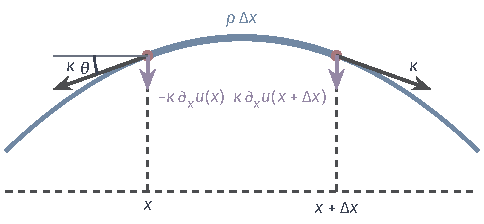
\includegraphics[width=81.975mm]{figures/06-differential-equations/02-partial-differential-equations/tikz/wave-string-element/figure.pdf}
  \caption{弦上一小段$[x,x+\Delta x]$的受力。蓝色粗线是这一小段，质量为$\rho\,\Delta x$。深灰箭头是两端沿切线的张力$\kappa$，紫色箭头是它们的竖直分量。这里弦向上凸，两个竖直分量都向下，合力把这一段拉回平衡位置。}
  \label{fig:wave-string-element}
\end{BookInlineFigure}

右端受到的竖直力是$\kappa\,\partial_xu(x+\Delta x,t)$，左端受到的是$-\kappa\,\partial_xu(x,t)$。再设单位质量上的竖直外力为$f(x,t)$。对这一小段用牛顿第二定律，得到
\[
 \rho\,\Delta x\,\partial_t^{2}u\approx\kappa\bigl[\partial_xu(x+\Delta x,t)-\partial_xu(x,t)\bigr]+\rho\,\Delta x\,f .
\]

两边除以$\rho\,\Delta x$，令$\Delta x\to0$，方括号除以$\Delta x$成为$\partial_x^{2}u$。于是得到一维波动方程：
\begin{equation}
 \partial_t^{2}u=c^{2}\partial_x^{2}u+f,\qquad c^{2}=\frac{\kappa}{\rho}.
 \label{eq:wave-string}
\end{equation}
常数$c>0$称为\term{波速}（wave speed）。量纲上$\kappa/\rho$的单位是$\mathrm{m^2/s^2}$，所以$c$确实是速度，后文会看到它正是扰动传播的速度。例如线密度$0.005\,\mathrm{kg/m}$、张力$80\,\mathrm{N}$的弦，$c=\sqrt{16000}\approx126.5\,\mathrm{m/s}$。张力越大、弦越轻，波跑得越快。

方程中的量各有含义，列在表~\ref{tab:wave-quantities}中。

\begin{BookInlineTable}
  \centering
  \caption{弦振动中各量的含义}
  \label{tab:wave-quantities}
  \begin{tabular}{lll}
    \toprule
    量 & 含义 & 在方程中的作用\\
    \midrule
    $u$ & 竖直位移 & 未知场\\
    $\partial_tu$ & 竖直速度 & 与位移一起构成状态\\
    $\partial_x^{2}u$ & 弦的弯曲 & 决定张力合力\\
    $c$ & 波速 & 把弯曲换算成加速度\\
    $f$ & 单位质量的外力 & 直接提供加速度\\
    \bottomrule
  \end{tabular}
\end{BookInlineTable}

\paragraph{弯曲决定加速度}
式~\eqref{eq:wave-string}和第~\ref{chap:diffusion-equations}章的热方程$\partial_tu=\partial_x^{2}u$右端相同，都是弯曲程度。区别只在左端：弯曲在热方程里决定变化的速度，在波动方程里决定变化的加速度。

这一个差别足以产生完全不同的运动。取初始形状$u_0=\mathrm{e}^{-x^{2}}$，$c=1$，波动问题的初速度为零。在$x=0$处，弯曲是$\partial_x^{2}u_0(0)=-2$。热方程的解在这一点的前期行为是下面左式，波动方程的解是右式：
\[
 u^{\mathrm{heat}}(0,t)\approx1-2t,\qquad u^{\mathrm{wave}}(0,t)\approx1-t^{2}.
\]

热方程中顶点一开始就以速度$2$下降，凡是向上凸的地方都立刻下降，凡是向下凹的地方都立刻上升，所以鼓包被抹平。弦的情形中，同样的弯曲只给出加速度，弦要积累速度才开始移动。一旦有了速度，弯曲消失后运动也不会停下，弦会冲过平衡位置。

图~\ref{fig:wave-curvature-acceleration}把这个差别画了出来。(a)的箭头是弯曲给出的量，(b)中热方程的鼓包逐渐变矮变宽并保持一个峰，(c)中波动方程的鼓包裂成了两个向外移动的峰。

\begin{BookInlineFigure}
  \centering
  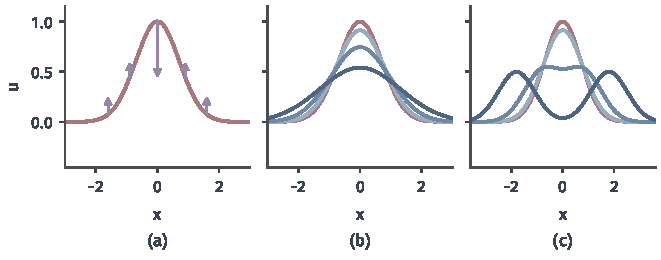
\includegraphics[width=112mm]{figures/06-differential-equations/02-partial-differential-equations/matplotlib/wave-curvature-acceleration/figure.pdf}
  \caption{同样的弯曲，两种后果。(a)初值$\mathrm{e}^{-x^{2}}$（红）和各点的弯曲$\partial_x^{2}u$（紫色箭头）。(b)热方程，蓝色由浅到深为$t=0.05,0.2,0.6$，弯曲作为速度，鼓包被抹平。(c)波动方程，$c=1$，初速度为零，蓝色由浅到深为$t=0.3,0.8,1.8$，弯曲作为加速度，鼓包裂成两个峰。}
  \label{fig:wave-curvature-acceleration}
\end{BookInlineFigure}

\paragraph{把弦看成珠链}
把函数看成很长的向量，可以把这个差别说得更具体。把弦换成$N$颗质量为$\rho h$的珠子，间距为$h$，相邻珠子之间由张力$\kappa$的轻线相连，如图~\ref{fig:wave-bead-chain}。第$j$颗珠子受到两侧的竖直拉力，分别正比于它与邻居的高度差除以$h$。

\begin{BookInlineFigure}
  \centering
  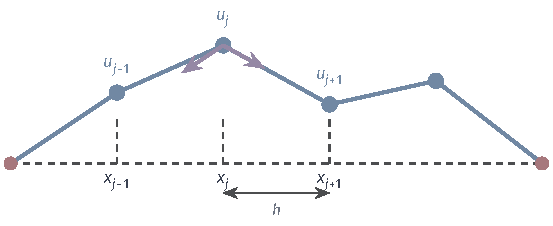
\includegraphics[width=93.606mm]{figures/06-differential-equations/02-partial-differential-equations/tikz/wave-bead-chain/figure.pdf}
  \caption{把弦换成珠链。珠子间距为$h$，两端（红点）固定。第$j$颗珠子受到两侧轻线的拉力（紫色箭头），竖直合力正比于$u_{j+1}-2u_j+u_{j-1}$，这正是二阶差分。}
  \label{fig:wave-bead-chain}
\end{BookInlineFigure}

列出第$j$颗珠子的牛顿第二定律，两端固定时取$u_0=u_{N+1}=0$，并除以质量，得到
\[
 \ddot{u}_j=c^{2}\,\frac{u_{j+1}-2u_j+u_{j-1}}{h^{2}},\qquad j=1,\ldots,N.
\]
记$\bm{u}=(u_1,\ldots,u_N)^\top$，$\bm{K}$为$h^{-2}$乘三对角矩阵$\mathrm{tridiag}(-1,2,-1)$，它对称正定。上式就是
\begin{equation}
 \ddot{\bm{u}}=-c^{2}\bm{K}\bm{u}.
 \label{eq:wave-chain}
\end{equation}

同样的空间离散用在热方程上，得到$\dot{\bm{u}}=-\bm{K}\bm{u}$。两个方程只差一阶时间导数，共用同一个矩阵$\bm{K}$。设$\bm{v}$是$\bm{K}$的特征向量，特征值为$\lambda>0$，把解限制在这个方向上，系数$a(t)$分别满足下面两个常微分方程：
\[
 \dot{a}=-\lambda a,\qquad \ddot{a}=-c^{2}\lambda a.
\]
前者给出衰减$\mathrm{e}^{-\lambda t}$，后者给出振荡$\cos(c\sqrt{\lambda}\,t)$。所以每个方向上一个是指数衰减，一个是不衰减的简谐振动，这是本章反复用到的对应。

这个类比也有失效的地方。珠链的频率有上限，这是因为特征值有上限；连续的弦可以振动得任意快。珠链上的扰动实际上以略低于$c$的速度散开，而连续弦上的波形不变。第~\ref{sec:wave-modes}节会用具体数字比较这些差别，波动方程的离散求解放在第~\ref{chap:pde-numerical-methods}章。

\paragraph{初始状态是一对函数}
式~\eqref{eq:wave-chain}的每个分量都是二阶常微分方程，要同时给位置和速度。连续的弦也一样，初始状态是一对函数：初始位移$u_0$和初始速度$u_1$。第~\ref{chap:pde-problems}章的例子正说明了这一点：$(0,1)$上$c=1$、两端固定时，$\cos(\pi t)\sin(\pi x)$和$(\cos\pi t+\sin\pi t)\sin(\pi x)$的初始位移相同，都是$\sin\pi x$，后续运动却不同。

把区域写成一般形式，本章的问题可以统一写出。

\begin{definition}[波动方程的初边值问题]
\label{def:wave-ibvp}
设$\Omega\subset\mathbb{R}^{d}$为区域，$c>0$，$T>0$。给定源项$f$、初始位移$u_0$和初始速度$u_1$。求$u(\bm{x},t)$满足
\begin{equation}
 \begin{aligned}
  \partial_t^{2}u-c^{2}\Delta u&=f && \text{于}\ \Omega\times(0,T],\\
  u(\cdot,0)=u_0,\quad\partial_tu(\cdot,0)&=u_1 && \text{于}\ \Omega,
 \end{aligned}
 \label{eq:wave-ibvp}
\end{equation}
以及边界$\partial\Omega\times(0,T]$上给定的边界条件。$\Omega=\mathbb{R}^{d}$时没有边界条件。
\end{definition}

\paragraph{端点怎样约束运动}
端点条件有两种基本类型，如图~\ref{fig:wave-boundary-types}。把弦的一端钉死，得到\term{固定端}（fixed end）$u=0$，端点没有位移，因而没有速度。把弦的一端系在一个能沿竖直光滑杆自由滑动的无质量小环上，得到\term{自由端}（free end）。小环在竖直方向不能受力，否则加速度无穷大，所以张力的竖直分量为零，即$\partial_xu=0$。

\begin{BookInlineFigure}
  \centering
  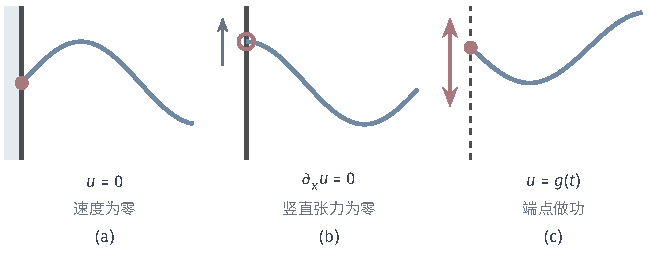
\includegraphics[width=109.703mm]{figures/06-differential-equations/02-partial-differential-equations/tikz/wave-boundary-types/figure.pdf}
  \caption{三种端点。(a)固定端：端点位移和速度为零。(b)自由端：小环沿光滑竖直杆滑动，弦在端点的切线水平。(c)驱动端：端点按给定的位移$g(t)$运动，并通过张力向弦做功。}
  \label{fig:wave-boundary-types}
\end{BookInlineFigure}

两种条件限制的量不同，共同点是端点不向弦输入能量。功率等于力乘速度。在端点上，支撑对弦的竖直力等于$\kappa\,\partial_{\bm{n}}u$，其中$\partial_{\bm{n}}$是外法向导数：右端是$\partial_x$，左端是$-\partial_x$。所以端点向弦输入的功率是
\begin{equation}
 P=\kappa\,\partial_{\bm{n}}u\,\partial_tu .
 \label{eq:wave-end-power}
\end{equation}

固定端让第二个因子$\partial_tu$为零，自由端让第一个因子$\partial_{\bm{n}}u$为零。两种方式都使$P=0$。如果端点按给定的位移运动，或者端点上施加给定的力，式~\eqref{eq:wave-end-power}一般不为零，能量就通过端点进出弦。表~\ref{tab:wave-boundary}总结了这四种情形。

\begin{BookInlineTable}
  \centering
  \caption{端点条件和端点功率}
  \label{tab:wave-boundary}
  \begin{tabular}{llll}
    \toprule
    端点 & 条件 & 被规定的量 & 功率$P$\\
    \midrule
    固定端 & $u=0$ & 位移和速度 & $0$\\
    自由端 & $\partial_{\bm{n}}u=0$ & 竖直力 & $0$\\
    位移驱动 & $u=g(t)$ & 位移和速度 & $\kappa\,\partial_{\bm{n}}u\,g'(t)$\\
    力驱动 & $\kappa\,\partial_{\bm{n}}u=g(t)$ & 竖直力 & $g(t)\,\partial_tu$\\
    \bottomrule
  \end{tabular}
\end{BookInlineTable}

初值和边值在角点处要彼此相容。位移驱动的左端$u(0,t)=g(t)$要有$C^{2}$解，必须满足下面三个条件，它们依次来自位移相等、速度相等和方程在角点处成立：
\[
 u_0(0)=g(0),\qquad u_1(0)=g'(0),\qquad g''(0)=c^{2}u_0''(0)+f(0,0).
\]
固定端是$g\equiv0$的情形。不相容时，间断或折角会从角点出发沿特征线传播，解只能在弱的意义下理解。


\section{一维传播公式}
\label{sec:wave-dalembert}

无界的弦上没有端点干扰，一维波动问题可以完全解出来。解的公式会回答两个问题：初始位移和初始速度各起什么作用，某一时空点的值究竟取决于哪段初值。

\paragraph{换坐标：沿两族直线看}
第~\ref{chap:pde-problems}章指出，一维波动方程的特征线是两族直线$x\pm ct=$常数。沿这两族直线取坐标，方程会变得非常简单。令
\[
 \xi=x-ct,\qquad \eta=x+ct,
\]
并把$u$写成$(\xi,\eta)$的函数。由链式法则，
\[
 \partial_x=\partial_\xi+\partial_\eta,\qquad \partial_t=c(\partial_\eta-\partial_\xi).
\]

把这两个算子分别平方再作差，混合项是唯一留下的部分：
\[
 \partial_t^{2}-c^{2}\partial_x^{2}=c^{2}(\partial_\eta-\partial_\xi)^{2}-c^{2}(\partial_\xi+\partial_\eta)^{2}=-4c^{2}\partial_\xi\partial_\eta .
\]
于是无源的波动方程等价于
\begin{equation}
 \partial_\xi\partial_\eta u=0.
 \label{eq:wave-characteristic-form}
\end{equation}

式~\eqref{eq:wave-characteristic-form}说$\partial_\eta u$不随$\xi$变化，只是$\eta$的函数。对$\eta$积分，积分“常数”是$\xi$的函数。所以$C^{2}$解都可以写成两个一元函数之和：
\begin{equation}
 u(x,t)=F(x-ct)+G(x+ct).
 \label{eq:wave-general-solution}
\end{equation}

$F(x-ct)$是形状$F$以速度$c$向右平移，$G(x+ct)$是形状$G$以速度$c$向左平移。这两项称为\term{行波}（travelling wave）。方程$\partial_t^{2}u=c^{2}\partial_x^{2}u$的全部解都由一列右行波和一列左行波叠加而成，两列波互相穿过，彼此不改变形状。

\paragraph{由初值确定两列波}
把式~\eqref{eq:wave-general-solution}代入两个初始条件，得到
\[
 F(x)+G(x)=u_0(x),\qquad -cF'(x)+cG'(x)=u_1(x).
\]
对第二式从$0$到$x$积分，再除以$c$，其中$K=G(0)-F(0)$是常数：
\[
 G(x)-F(x)=\frac1c\int_0^{x}u_1(s)\,\mathrm{d}s+K .
\]

把它与第一式相加减，就解出了两个函数：
\[
 \begin{aligned}
  F(x)&=\frac12u_0(x)-\frac1{2c}\int_0^{x}u_1(s)\,\mathrm{d}s-\frac K2,\\
  G(x)&=\frac12u_0(x)+\frac1{2c}\int_0^{x}u_1(s)\,\mathrm{d}s+\frac K2 .
 \end{aligned}
\]
代回式~\eqref{eq:wave-general-solution}，常数$K$相消，两个积分合并成从$x-ct$到$x+ct$的积分。这样就得到了下面的公式。

\begin{theorem}[\term{d'Alembert公式}（d'Alembert formula）]
\label{thm:wave-dalembert}
设$u_0\in C^{2}(\mathbb{R})$，$u_1\in C^{1}(\mathbb{R})$。一维问题$\partial_t^{2}u=c^{2}\partial_x^{2}u$，$u(\cdot,0)=u_0$，$\partial_tu(\cdot,0)=u_1$在$\mathbb{R}\times[0,\infty)$上有唯一的$C^{2}$解
\begin{equation}
 u(x,t)=\frac12\bigl[u_0(x-ct)+u_0(x+ct)\bigr]+\frac1{2c}\int_{x-ct}^{x+ct}u_1(s)\,\mathrm{d}s .
 \label{eq:wave-dalembert}
\end{equation}
\end{theorem}

\begin{proof}
先证唯一性。设$u$是$C^{2}$解，换到坐标$(\xi,\eta)$后，$t\geq0$对应区域$\eta\geq\xi$。这个区域在两个坐标方向上的截线都是连通的半直线，所以式~\eqref{eq:wave-characteristic-form}可以如上逐次积分，得到式~\eqref{eq:wave-general-solution}。前面的代入过程说明$F,G$由初值确定到相差一个相消的常数，因此$u$必定是式~\eqref{eq:wave-dalembert}。

再证式~\eqref{eq:wave-dalembert}确实是解。记$x_-=x-ct$，$x_+=x+ct$。由链式法则和变上限积分的求导公式，对$x$求两次，得到
\[
 \partial_x^{2}u=\frac12\bigl[u_0''(x_-)+u_0''(x_+)\bigr]+\frac1{2c}\bigl[u_1'(x_+)-u_1'(x_-)\bigr].
\]

对$t$求一次，$x_\pm$对$t$的导数是$\pm c$，于是
\[
 \partial_tu=\frac c2\bigl[-u_0'(x_-)+u_0'(x_+)\bigr]+\frac12\bigl[u_1(x_+)+u_1(x_-)\bigr].
\]

再对$t$求一次，得到
\[
 \partial_t^{2}u=\frac{c^{2}}2\bigl[u_0''(x_-)+u_0''(x_+)\bigr]+\frac c2\bigl[u_1'(x_+)-u_1'(x_-)\bigr].
\]
比较前后两式，$\partial_t^{2}u=c^{2}\partial_x^{2}u$。题设的光滑性保证这些导数都连续。令$t=0$，$x_-=x_+=x$，积分项为零，$u=u_0$；$\partial_tu$的表达式给出$\partial_tu=u_1$。
\end{proof}

用一组光滑的数据验证公式。取$c=2$，$u_0=\sin x$，$u_1=\cos x$。式~\eqref{eq:wave-dalembert}的两项分别是
\[
 \begin{aligned}
  \frac12\bigl[\sin(x-2t)+\sin(x+2t)\bigr]&=\sin x\cos2t,\\
  \frac14\int_{x-2t}^{x+2t}\cos s\,\mathrm{d}s&=\frac12\cos x\sin2t .
 \end{aligned}
\]
两者之和满足$\partial_t^{2}u=-4u=4\partial_x^{2}u$，$t=0$时位移是$\sin x$，速度是$\cos x$。

式~\eqref{eq:wave-dalembert}有两项，分别来自初始位移和初始速度。由线性性，可以把它们分开讨论。

\paragraph{初始位移的贡献}
取$c=1$，初速度为零，初始位移是帐篷形
\[
 u_0(x)=\Lambda(x)=\max\{1-\lvert x\rvert,\,0\}.
\]
式~\eqref{eq:wave-dalembert}只剩第一项，解是
\begin{equation}
 u(x,t)=\frac12\bigl[\Lambda(x-t)+\Lambda(x+t)\bigr].
 \label{eq:wave-tent-solution}
\end{equation}
帐篷在$0,\pm1$处有折角，严格说来不是$C^{2}$函数，式~\eqref{eq:wave-tent-solution}在折角运动的线上没有二阶导数，它是第~\ref{chap:pde-problems}章意义下的弱解，可以看成光滑初值的解的极限。

式~\eqref{eq:wave-tent-solution}说，初始鼓包分成高度减半的两份，一份向右，一份向左。取$t=1/2$，手算几个点的值：
\[
 \begin{aligned}
  u(0,\tfrac12)&=\tfrac12[\Lambda(-\tfrac12)+\Lambda(\tfrac12)]=\tfrac12,\\
  u(\tfrac12,\tfrac12)&=\tfrac12[\Lambda(0)+\Lambda(1)]=\tfrac12,\\
  u(1,\tfrac12)&=\tfrac12[\Lambda(\tfrac12)+\Lambda(\tfrac32)]=\tfrac14 .
 \end{aligned}
\]
此时两份还重叠着，叠加成高度$1/2$的平台。到$t=1$，两份恰好分开；到$t=2$，它们的中心分别在$\pm2$，中间的弦回到零位，如图~\ref{fig:wave-dalembert-displacement}。

\begin{BookInlineFigure}
  \centering
  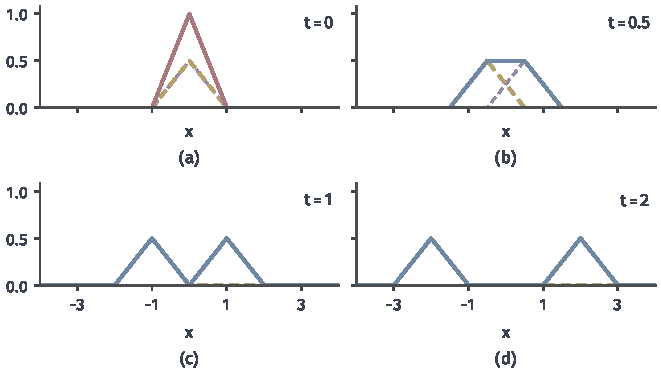
\includegraphics[width=112mm]{figures/06-differential-equations/02-partial-differential-equations/matplotlib/wave-dalembert-displacement/figure.pdf}
  \caption{帐篷形初始位移（$c=1$，初速度为零）在四个时刻的解。黄色虚线是左行波$\frac12\Lambda(x+t)$，紫色虚线是右行波$\frac12\Lambda(x-t)$，实线是两者之和。鼓包分成两半后互不干扰，形状和高度此后不再改变。}
  \label{fig:wave-dalembert-displacement}
\end{BookInlineFigure}

注意帐篷的折角也被带走了。原来的三个折角各分裂成两个，分别沿特征线运动，没有任何一个被磨圆。对比热方程，折角在任意正时刻都消失。波动方程的解在时刻$t$和初值一样光滑，不会更光滑。

\paragraph{初始速度的贡献}
再取初始位移为零，用小锤敲打区间$(-1,1)$，即$c=1$，$u_1=\mathbb{I}\{\lvert x\rvert<1\}$。式~\eqref{eq:wave-dalembert}只剩积分项，被积函数只在$(-1,1)$上不为零，所以
\begin{equation}
 u(x,t)=\frac12\,\bigl\lvert(x-t,\,x+t)\cap(-1,1)\bigr\rvert .
 \label{eq:wave-box-solution}
\end{equation}
竖线表示区间的长度。这个函数连续，但$u_1$的跳跃使它不是$C^{2}$函数，它同样在弱的意义下解方程。

固定一个位置观察。在$x=0$处，式~\eqref{eq:wave-box-solution}的交集在$t\leq1$时是$(-t,t)$，在$t\geq1$时是$(-1,1)$，于是
\[
 u(0,t)=\min\{t,\,1\}.
\]
位移先线性上升，到$t=1$后停在$1$，再也不回来。

固定一个时刻观察。取$t=3$，在几个点上读出交集的长度：
\[
 u(0,3)=\tfrac12\cdot2=1,\qquad u(3,3)=\tfrac12\cdot1=\tfrac12,\qquad u(4,3)=0.
\]
解是一个梯形：在$\lvert x\rvert\leq t-1$上高度为$1$，在$\lvert x\rvert=t+1$处降到零。图~\ref{fig:wave-dalembert-velocity}显示这个梯形不断变宽，高度不变。

\begin{BookInlineFigure}
  \centering
  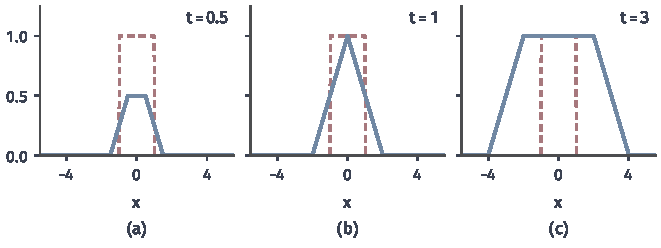
\includegraphics[width=112mm]{figures/06-differential-equations/02-partial-differential-equations/matplotlib/wave-dalembert-velocity/figure.pdf}
  \caption{初始速度为$(-1,1)$的指示函数（红色虚线）时三个时刻的解（蓝），$c=1$，初始位移为零。解是逐渐变宽的梯形，中间的平台高度为$1$，$t>1$后不再升高。}
  \label{fig:wave-dalembert-velocity}
\end{BookInlineFigure}

为什么速度的贡献是积分？设想只在一点$y$附近的小区间$\mathrm{d}y$上有初速度。式~\eqref{eq:wave-dalembert}的积分说，$\lvert x-y\rvert<ct$的点得到位移$u_1(y)\,\mathrm{d}y/(2c)$，更远的点还没有收到信号。一次局部的推动在波前走过的范围内留下固定的抬高，所有$y$的贡献加起来就是积分。

这和初始位移的情形不同。位移的两半走开后，中间恢复零位；速度的作用却留下永久的位移，因为被敲过的弦有净动量。对空间积分可以把这件事算清楚。由式~\eqref{eq:wave-box-solution}，$\int_{\mathbb{R}}\partial_tu\,\mathrm{d}x$保持为初值的积分$2$，所以
\[
 \int_{\mathbb{R}}u(x,t)\,\mathrm{d}x=2t.
\]
梯形的面积正是这样增长的：宽度每单位时间增加$2$，高度为$1$。

\paragraph{一个时空点依赖哪段初值}
式~\eqref{eq:wave-dalembert}直接告诉我们计算$u(x_0,t_0)$要用到什么：$u_0$只用到两个端点$x_0\pm ct_0$，$u_1$用到整个区间$[x_0-ct_0,x_0+ct_0]$。从点$(x_0,t_0)$沿两条特征线回溯到$t=0$，就截出这个区间，如图~\ref{fig:wave-dependence}(a)。

反过来，初值在区间$[a,b]$上的变化只能影响图~\ref{fig:wave-dependence}(b)的阴影区域，$a-ct\leq x\leq b+ct$，以外的点完全不受影响。扰动以速度$c$向两侧扩展。

\begin{BookInlineFigure}
  \centering
  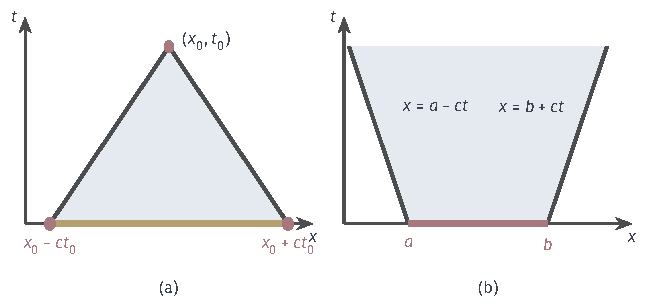
\includegraphics[width=109.647mm]{figures/06-differential-equations/02-partial-differential-equations/tikz/wave-dependence/figure.pdf}
  \caption{一维波动方程的依赖关系。(a)点$(x_0,t_0)$的值由两条特征线（深灰）截出的区间决定：两个红点是所用的位移，黄色线段是所用的速度。(b)初始数据$[a,b]$（红色线段）的变化只能影响阴影区域。}
  \label{fig:wave-dependence}
\end{BookInlineFigure}

用前面的两个例子走一遍。取$c=1$，$(x_0,t_0)=(1/2,2)$，依赖区间是$[-3/2,5/2]$。帐篷初始位移只用到$u_0(-3/2)$和$u_0(5/2)$，两者都为零，于是
\[
 u(\tfrac12,2)=0.
\]
帐篷的两半都已经从这里经过。小锤初始速度要用整个依赖区间，其中包含$(-1,1)$，于是
\[
 u(\tfrac12,2)=\tfrac12\cdot2=1.
\]
如果把初值在$x=3$附近改掉，这两个数都不变，因为$3$不在依赖区间内。

图~\ref{fig:wave-spacetime}把两个例子画在时空平面上。(a)中的折角沿特征线运动，帐篷走后留下空白；(b)中两列波前沿之间的弦保持抬高。

\begin{BookInlineFigure}
  \centering
  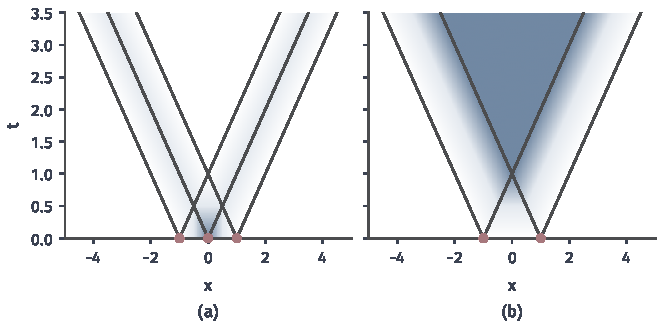
\includegraphics[width=112mm]{figures/06-differential-equations/02-partial-differential-equations/matplotlib/wave-spacetime/figure.pdf}
  \caption{时空平面上的解，$c=1$，颜色越深$u$越大。(a)帐篷形初始位移。(b)$(-1,1)$上的初始速度。深灰直线是从初始数据的折点（红点）出发的特征线，解的不光滑处全部落在这些线上。}
  \label{fig:wave-spacetime}
\end{BookInlineFigure}

\paragraph{解对初值的连续依赖}
由式~\eqref{eq:wave-dalembert}，把两项分别放大，得到点态估计
\begin{equation}
 \sup_{x}\lvert u(x,t)\rvert\leq\sup_{x}\lvert u_0(x)\rvert+t\,\sup_{x}\lvert u_1(x)\rvert .
 \label{eq:wave-sup-bound}
\end{equation}
线性问题中，把它用在两组数据之差上，就得到连续依赖：在有限时间$[0,T]$内，数据的小扰动只造成解的小扰动。

式~\eqref{eq:wave-sup-bound}右端随$t$线性增长，这不是估计不够好。$u_1\equiv1$，$u_0\equiv0$时解是$u=t$，恰好取到等号。这也说明这个估计只在有限时间上有用，长时间的稳定性要另行讨论。

\paragraph{粗糙初值的解}
帐篷和指示函数都不满足定理~\ref{thm:wave-dalembert}的光滑性条件，式~\eqref{eq:wave-dalembert}给出的函数在什么意义下是解？第~\ref{chap:pde-problems}章的回答是弱解：对任意紧支在$\mathbb{R}\times(0,\infty)$中的光滑函数$\varphi$，要求
\begin{equation}
 \iint u\,\bigl(\partial_t^{2}\varphi-c^{2}\partial_x^{2}\varphi\bigr)\,\mathrm{d}x\,\mathrm{d}t=0 .
 \label{eq:wave-weak}
\end{equation}
经典解通过两次分部积分满足它，而式~\eqref{eq:wave-weak}中不再出现$u$的导数。

设$u_0$连续，$u_1$局部可积。取光滑函数列$u_0^{(m)}\to u_0$（在紧集上一致）、$u_1^{(m)}\to u_1$（局部$L^1$），对应的光滑解$u^{(m)}$满足式~\eqref{eq:wave-weak}。把式~\eqref{eq:wave-dalembert}的两项放大，$u^{(m)}$在紧集上一致收敛到由同一公式给出的$u$，于是极限也满足式~\eqref{eq:wave-weak}。这说明$\Lambda$的解和小锤的解是光滑解的极限，式~\eqref{eq:wave-tent-solution}和式~\eqref{eq:wave-box-solution}的说法是合理的。


\section{边界模式}
\label{sec:wave-modes}

弦总有端点，波跑到端点后会怎样？半直线上用反射就能回答，有界区间上波来回反射，解的结构要用模式描述。边界条件决定可用的模式，这一点和第~\ref{chap:diffusion-equations}章相同，时间因子却完全不同。

\paragraph{半直线：固定端的翻转反射}
考虑$x>0$上的弦，端点$x=0$固定。d'Alembert公式需要整条实轴上的数据，我们把初值延拓到$x<0$上，让解自动在$x=0$处为零。如果实轴上的数据关于原点是奇函数，解也是奇函数，因为$-u(-x,t)$满足同样的问题，由唯一性等于$u$；奇函数在$0$处的值只能是$0$。

于是对$u_0,u_1$作\term{奇延拓}（odd extension）：$x<0$时令$u_0(x)=-u_0(-x)$，$u_1(x)=-u_1(-x)$。这是在墙的另一侧放一个翻转的镜像。把延拓后的数据代入式~\eqref{eq:wave-dalembert}，分情况计算。当$x\geq ct$时，$x-ct\geq0$，用不到延拓，公式不变。当$0\leq x<ct$时，$u_0(x-ct)=-u_0(ct-x)$，积分中$(x-ct,\,ct-x)$是对称区间，奇函数的积分为零。

这样就得到半直线固定端的解：
\begin{equation}
 u(x,t)=
 \begin{cases}
  \dfrac12\bigl[u_0(x-ct)+u_0(x+ct)\bigr]+\dfrac1{2c}\displaystyle\int_{x-ct}^{x+ct}u_1\,\mathrm{d}s, & x\geq ct,\\
  \dfrac12\bigl[u_0(ct+x)-u_0(ct-x)\bigr]+\dfrac1{2c}\displaystyle\int_{ct-x}^{ct+x}u_1\,\mathrm{d}s, & 0\leq x<ct .
 \end{cases}
 \label{eq:wave-halfline-fixed}
\end{equation}
第二行中，$-\frac12u_0(ct-x)$是从左侧镜像传来的、已经翻转的反射波。

\paragraph{半直线：自由端的同号反射}
自由端要求$\partial_xu(0,t)=0$。偶函数的导数在$0$处为零，所以改作\term{偶延拓}（even extension）：$u_0(-x)=u_0(x)$，$u_1(-x)=u_1(x)$。镜像不翻转。同样的计算在$0\leq x<ct$时给出
\begin{equation}
 u(x,t)=\frac12\bigl[u_0(ct+x)+u_0(ct-x)\bigr]+\frac1{2c}\Bigl[\int_0^{ct+x}u_1\,\mathrm{d}s+\int_0^{ct-x}u_1\,\mathrm{d}s\Bigr],
 \label{eq:wave-halfline-free}
\end{equation}
$x\geq ct$时仍是式~\eqref{eq:wave-dalembert}。

这两个公式要成为$C^{2}$解，延拓后的数据必须足够光滑。固定端要求$u_0(0)=u_0''(0)=u_1(0)=0$，这正是表~\ref{tab:wave-boundary}之后的相容条件在$g\equiv0$、$f\equiv0$时的结果。自由端要求$u_0'(0)=u_1'(0)=0$。解也是唯一的：若$u$是半直线上固定端的$C^{2}$解，由方程得$\partial_x^{2}u(0,t)=c^{-2}\partial_t^{2}u(0,t)=0$，它的奇延拓在实轴上是$C^{2}$解，再用定理~\ref{thm:wave-dalembert}；自由端用偶延拓同理。

\paragraph{走一遍反射}
取$c=1$，$u_1=0$，初始位移是中心在$x=3$的帐篷$\Lambda(x-3)$。它分成两半，右行的一半直接走开，左行的一半$\frac12\Lambda(x-3+t)$在$t=2$时到达端点，$t=3$时中心位于端点。

在反射发生的时刻，两种端点表现最为不同。取$t=3$，靠近端点$0\leq x\leq1$处的解由式~\eqref{eq:wave-halfline-fixed}和式~\eqref{eq:wave-halfline-free}算出：
\[
 u^{\mathrm{fix}}(x,3)=\tfrac12[\Lambda(x)-\Lambda(-x)]=0,\qquad u^{\mathrm{free}}(x,3)=\Lambda(x).
\]
固定端附近入射波和镜像恰好抵消，位移为零，能量此时全在速度里；自由端附近两者相加，端点位移翻倍，高度达到$1$。

反射之后再取一点比较。在$(x,t)=(1,\,7/2)$处，$ct+x=9/2$，$ct-x=5/2$，代入两个公式：
\[
 u^{\mathrm{fix}}(1,\tfrac72)=\tfrac12[\Lambda(\tfrac32)-\Lambda(-\tfrac12)]=-\tfrac14,\qquad u^{\mathrm{free}}(1,\tfrac72)=\tfrac14 .
\]
固定端反射回来的波被翻转，自由端反射回来的波保持同号，如图~\ref{fig:wave-reflection}。

\begin{BookInlineFigure}
  \centering
  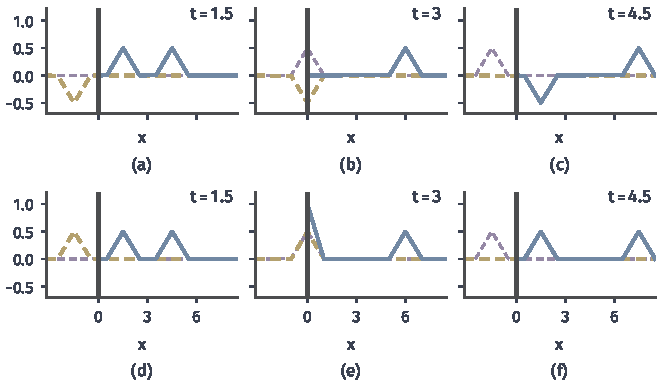
\includegraphics[width=112mm]{figures/06-differential-equations/02-partial-differential-equations/matplotlib/wave-reflection/figure.pdf}
  \caption{半直线上$\Lambda(x-3)$的两半波在端点（深灰竖线）的反射，$c=1$。上排是固定端，下排是自由端。紫色虚线是左行的入射波，黄色虚线是从$x<0$一侧传来的镜像，上排翻转，下排不翻转。蓝线是$x\geq0$上的解，等于两者与右行波之和。}
  \label{fig:wave-reflection}
\end{BookInlineFigure}

\paragraph{区间：分离变量}
现在考虑$(0,L)$上的弦。波在两端之间来回反射，用镜像可以写出来，但更好的办法是换一个角度：寻找形状不变、只有幅度随时间变化的解。设$u(x,t)=X(x)\Theta(t)$，代入$\partial_t^{2}u=c^{2}\partial_x^{2}u$并除以$c^{2}X\Theta$，得到
\[
 \frac{\ddot{\Theta}(t)}{c^{2}\Theta(t)}=\frac{X''(x)}{X(x)}.
\]

左边只依赖$t$，右边只依赖$x$，所以两边等于同一个常数，记作$-\lambda$。这种做法称为\term{分离变量法}（separation of variables）。空间部分是特征值问题，时间部分是简谐振子：
\begin{equation}
 -X''=\lambda X,\qquad \ddot{\Theta}=-c^{2}\lambda\,\Theta .
 \label{eq:wave-separation}
\end{equation}

边界条件落在$X$上。先看两端固定的情形，$X(0)=X(L)=0$。把$X$乘上式并积分，分部积分后边界项为零：
\[
 \lambda\int_0^{L}X^{2}\,\mathrm{d}x=\int_0^{L}(X')^{2}\,\mathrm{d}x .
\]
非零的$X$不可能是常数（它要在端点取零），所以$\lambda>0$。记$\lambda=k^{2}$，$k>0$，通解是$X=A\cos kx+B\sin kx$。条件$X(0)=0$给出$A=0$，条件$X(L)=0$给出$\sin kL=0$，于是
\begin{equation}
 k_n=\frac{n\pi}{L},\qquad X_n(x)=\sin\frac{n\pi x}{L},\qquad n=1,2,\ldots
 \label{eq:wave-dirichlet-modes}
\end{equation}

时间部分的频率是$\omega_n=ck_n=cn\pi/L$，称为第$n$个\term{固有频率}（natural frequency）。

其他端点组合做同样的计算，只是条件换了，结果列在表~\ref{tab:wave-modes}中，前三个模式画在图~\ref{fig:wave-mode-shapes}中。两端自由时多出$\lambda=0$的常数模式，它的时间因子是$a+bt$：整根弦没有受到任何拉回的力，可以整体匀速平移。一端固定一端自由时，$X$在固定端为零、在自由端斜率为零，波长的四分之一装进弦长，所以$k$是$\pi/(2L)$的奇数倍。

\begin{BookInlineTable}
  \centering
  \caption{区间$(0,L)$上三种端点组合的空间模式}
  \label{tab:wave-modes}
  \begin{tabular}{lll}
    \toprule
    端点 & $X_n$ & $k_n$\\
    \midrule
    固定--固定 & $\sin(n\pi x/L)$ & $n\pi/L$，$n\geq1$\\
    自由--自由 & $\cos(n\pi x/L)$ & $n\pi/L$，$n\geq0$\\
    固定--自由 & $\sin((n-\tfrac12)\pi x/L)$ & $(n-\tfrac12)\pi/L$，$n\geq1$\\
    \bottomrule
  \end{tabular}
\end{BookInlineTable}

\begin{BookInlineFigure}
  \centering
  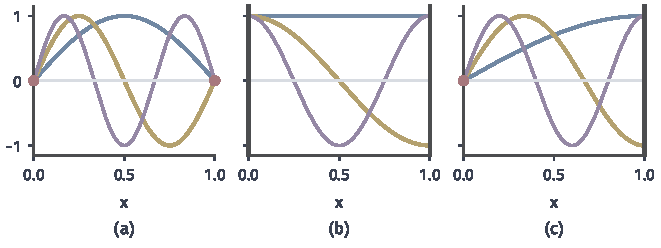
\includegraphics[width=112mm]{figures/06-differential-equations/02-partial-differential-equations/matplotlib/wave-mode-shapes/figure.pdf}
  \caption{$L=1$时的前三个空间模式，蓝、黄、紫依次为$n$增大。红点表示固定端（$X=0$），深灰粗竖线表示自由端（$X'=0$）。(a)固定--固定。(b)自由--自由，蓝线是常数模式。(c)固定--自由。}
  \label{fig:wave-mode-shapes}
\end{BookInlineFigure}

\paragraph{模式展开的解}
两端固定时，由式~\eqref{eq:wave-separation}和线性性，把所有模式叠加起来。把初值按$\sin(n\pi x/L)$展开，系数是
\begin{equation}
 a_n=\frac2L\int_0^{L}u_0(x)\sin\frac{n\pi x}{L}\,\mathrm{d}x,\qquad b_n=\frac2L\int_0^{L}u_1(x)\sin\frac{n\pi x}{L}\,\mathrm{d}x .
 \label{eq:wave-coefficients}
\end{equation}
这组正弦函数在$L^{2}(0,L)$中正交而且完备，这是Fourier级数理论的结果，可参考\BookChapterRef{chap:fourier-transform}{卷四第14章“Fourier变换”}。下面的定理说明，数据足够光滑时级数给出经典解。

\begin{theorem}[两端固定的模式解]
\label{thm:wave-series}
设$u_0\in C^{3}[0,L]$，$u_1\in C^{2}[0,L]$，并满足在$x=0,L$处$u_0=u_0''=0$，$u_1=0$。记$\omega_n=cn\pi/L$，系数由式~\eqref{eq:wave-coefficients}给出，则
\begin{equation}
 u(x,t)=\sum_{n=1}^{\infty}\Bigl(a_n\cos\omega_nt+\frac{b_n}{\omega_n}\sin\omega_nt\Bigr)\sin\frac{n\pi x}{L}
 \label{eq:wave-series}
\end{equation}
是$[0,L]\times[0,\infty)$上的$C^{2}$函数，满足$\partial_t^{2}u=c^{2}\partial_x^{2}u$、两端为零和两个初始条件。
\end{theorem}

\begin{proof}
关键是系数衰减得足够快，使逐项求两次导后的级数一致收敛。记$k_n=n\pi/L$。对$a_n$的积分分部三次：前两次的边界项因$u_0$和$u_0''$在端点为零而消失，第三次仍保留积分。于是
\[
 a_n=-\frac{1}{k_n^{3}}\cdot\frac2L\int_0^{L}u_0'''(x)\cos k_nx\,\mathrm{d}x .
\]

右端的积分是$u_0'''$关于余弦系的系数，由Bessel不等式，这些系数平方可和，所以$(n^{3}a_n)$属于$\ell^{2}$。同样对$b_n$分部两次，$(n^{2}b_n)$属于$\ell^{2}$。由Cauchy--Schwarz不等式，
\[
 \sum_{n}n^{2}\lvert a_n\rvert=\sum_{n}\frac{n^{3}\lvert a_n\rvert}{n}\leq\Bigl(\sum_{n}n^{6}a_n^{2}\Bigr)^{1/2}\Bigl(\sum_{n}\frac1{n^{2}}\Bigr)^{1/2}<\infty,
\]
同理$\sum_nn\lvert b_n\rvert<\infty$。

式~\eqref{eq:wave-series}的通项及其对$x,t$的至多二阶偏导，绝对值都不超过常数乘$n^{2}\lvert a_n\rvert+n\lvert b_n\rvert$。由Weierstrass判别法，这些级数都一致收敛，可以逐项求导，所以$u$是$C^{2}$函数。每一项都满足方程和边界条件，因而$u$也满足。令$t=0$，由余弦和正弦展开的收敛性，得到两个初始条件。
\end{proof}

式~\eqref{eq:wave-series}的解也是唯一的，这要等第~\ref{sec:wave-energy}节用能量证明。数据不够光滑时，只要$(u_0,u_1)\in H_0^{1}(0,L)\times L^{2}(0,L)$，级数仍在能量的意义下收敛，所得的函数是弱解，折线初值就属于这种情形。

自由端的常数模式可以手算验证。取$L=1$，$c=1$，两端自由，$u_0=0$，$u_1=1+\cos\pi x$。把$u_1$看成常数模式和第一个余弦模式之和，常数模式的时间因子是$t$，第一个模式的时间因子是$\sin(\pi t)/\pi$，所以
\[
 u(x,t)=t+\frac{\sin\pi t}{\pi}\cos\pi x .
\]
代入可得
\[
 \partial_t^{2}u=-\pi\sin(\pi t)\cos\pi x=\partial_x^{2}u .
\]
两端$\partial_xu=0$，$t=0$时位移为零，速度是$u_1$。第一项让弦整体匀速上升，第二项是叠加在上面的振动，这是固定端不会出现的现象。

\paragraph{驻波是两列行波之和}
式~\eqref{eq:wave-series}的每一项称为\term{驻波}（standing wave）：形状不变，只是幅度随时间振荡，节点永远不动。这看起来和行波毫无关系。其实由积化和差，
\begin{equation}
 \cos(ckt)\sin(kx)=\frac12\bigl[\sin k(x-ct)+\sin k(x+ct)\bigr].
 \label{eq:wave-standing}
\end{equation}

一个驻波就是一列右行波和一列左行波的叠加，这正是式~\eqref{eq:wave-general-solution}的形式。两列波不断反射，在区间内干涉出固定的形状。图~\ref{fig:wave-standing-traveling}用$L=1$，$c=1$，$n=1$画出了这个分解。

\begin{BookInlineFigure}
  \centering
  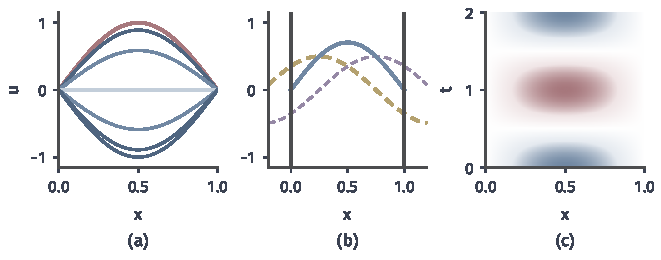
\includegraphics[width=112mm]{figures/06-differential-equations/02-partial-differential-equations/matplotlib/wave-standing-traveling/figure.pdf}
  \caption{第一个驻波$\cos(\pi t)\sin(\pi x)$，$L=1$，$c=1$。(a)不同时刻的形状，红色是$t=0$，端点始终为零。(b)$t=0.25$的分解：黄色虚线是左行波，紫色虚线是右行波，蓝线是两者之和，它在两端（深灰竖线）为零。(c)时空热图，蓝为正，红为负，$t=1$附近弦完全翻转。}
  \label{fig:wave-standing-traveling}
\end{BookInlineFigure}

把这个观察用到整个级数上。对式~\eqref{eq:wave-series}逐项用式~\eqref{eq:wave-standing}，并把$u_0,u_1$作奇延拓后再以$2L$为周期延拓到实轴，得到的正是d'Alembert公式
\begin{equation}
 u(x,t)=\frac12\bigl[\tilde{u}_0(x-ct)+\tilde{u}_0(x+ct)\bigr]+\frac1{2c}\int_{x-ct}^{x+ct}\tilde{u}_1(s)\,\mathrm{d}s .
 \label{eq:wave-interval-extension}
\end{equation}
其中$\tilde{u}_0,\tilde{u}_1$是延拓后的函数。奇延拓保证$x=0$处为零，以$2L$为周期再关于$x=L$也是奇的，所以$x=L$处也为零。这就是在两堵墙之间反复照镜子：反射和模式是同一个解的两种写法。式~\eqref{eq:wave-interval-extension}说明解沿时间有周期$2L/c$，一个波跑到对端再回来刚好用这么长时间。

\paragraph{手算：拨弦的模式}
取$L=1$，$c=1$，初速度为零，把中点拉起成折线$u_0=\min\{x,1-x\}$。由式~\eqref{eq:wave-coefficients}，分部积分后，正弦系数是
\begin{equation}
 a_n=\frac{4}{n^{2}\pi^{2}}\sin\frac{n\pi}{2}.
 \label{eq:wave-pluck-coefficients}
\end{equation}
$n$为偶数时$a_n=0$，这是因为折线关于中点对称，而偶数模式关于中点反对称。前三个非零系数是
\[
 a_1=\frac4{\pi^{2}}\approx0.405,\qquad a_3=-\frac4{9\pi^{2}}\approx-0.045,\qquad a_5=\frac4{25\pi^{2}}\approx0.016 .
\]

解是$u=\sum_na_n\cos(n\pi t)\sin(n\pi x)$。我们用两个时刻核对。在$t=1/2$、$x=1/2$处，奇数$n$的$\cos(n\pi/2)=0$，所以$u(\frac12,\frac12)=0$。用奇周期延拓的d'Alembert公式算，$x\mp t$是$0$和$1$，延拓函数在这两点都是零，结果相同。

在$t=1$时，$\cos(n\pi)=-1$（$n$为奇数），于是$u(x,1)=-u_0(x)$，弦完全翻转。$t=2$时回到初值，运动的周期是$2L/c=2$。图~\ref{fig:wave-plucked-series}的(a)是部分和，三项之后已接近折线，只是尖角处收敛慢；(b)(c)显示折角一直存在，并沿着反射的特征线来回移动。

\begin{BookInlineFigure}
  \centering
  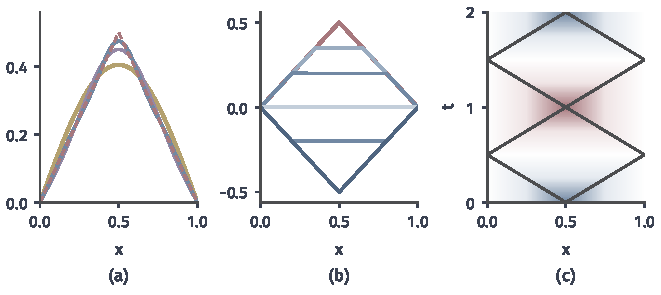
\includegraphics[width=112mm]{figures/06-differential-equations/02-partial-differential-equations/matplotlib/wave-plucked-series/figure.pdf}
  \caption{中点拨起的弦，$L=1$，$c=1$，$u_0=\min\{x,1-x\}$。(a)正弦级数的部分和，黄、紫、蓝分别取到$n=1,3,7$，红色虚线是$u_0$。(b)解的快照，红色是$t=0$，蓝色深浅为$t=0.15,0.3,0.5,0.7,1$，$t=1$时弦完全翻转。(c)时空热图（蓝正红负），深灰折线是在端点反射的特征线，也是折角的轨迹。}
  \label{fig:wave-plucked-series}
\end{BookInlineFigure}

\paragraph{时间因子：振荡与衰减}
同样的空间模式，在第~\ref{chap:diffusion-equations}章的热方程$\partial_tu=\partial_x^{2}u$中，第$n$个模式的时间因子是$\mathrm{e}^{-n^{2}\pi^{2}t}$（$L=1$），在波动方程中是$\cos(n\pi t)$（$c=1$）。图~\ref{fig:wave-heat-mode-factor}并排画出了前三个因子。

热方程的高频模式衰减极快，这就是折角瞬间消失的原因。波动方程的高频模式幅度完全不变，只是振荡得更快。所以波动方程不会平滑初值，初值的高频成分永远留在解里。

\begin{BookInlineFigure}
  \centering
  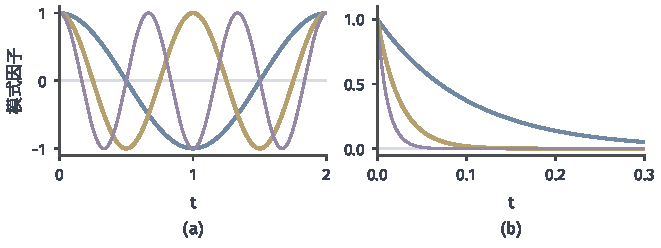
\includegraphics[width=112mm]{figures/06-differential-equations/02-partial-differential-equations/matplotlib/wave-heat-mode-factor/figure.pdf}
  \caption{第$n$个模式的时间因子，$L=1$，蓝、黄、紫依次为$n=1,2,3$。(a)波动方程$\cos(n\pi t)$，$c=1$，幅度不衰减。(b)热方程$\mathrm{e}^{-n^{2}\pi^{2}t}$，模式越高衰减越快（注意时间轴范围不同）。}
  \label{fig:wave-heat-mode-factor}
\end{BookInlineFigure}

\paragraph{离散的模式}
回到式~\eqref{eq:wave-chain}的珠链，看模式如何从有限维走到无限维。设$L=1$，$c=1$，有$N$颗珠子，$h=1/(N+1)$。$\bm{K}$的特征向量正是在格点上取值的$\sin(k\pi x)$，特征值和频率是
\begin{equation}
 \lambda_k=\frac4{h^{2}}\sin^{2}\frac{k\pi h}{2},\qquad \omega_k=\sqrt{\lambda_k}=\frac2h\sin\frac{k\pi h}{2},\qquad k=1,\ldots,N.
 \label{eq:wave-chain-frequencies}
\end{equation}

$N=3$，$h=1/4$时，三个频率和连续弦的$n\pi$比较如下：
\[
 \begin{aligned}
  \text{珠链：}\quad&\omega_1\approx3.06,\quad\omega_2\approx5.66,\quad\omega_3\approx7.39,\\
  \text{连续弦：}\quad&\pi\approx3.14,\quad2\pi\approx6.28,\quad3\pi\approx9.42.
 \end{aligned}
\]
最低的模式已经很准，最高的模式误差最大。图~\ref{fig:wave-discrete-modes}(a)显示珠链的特征向量恰好是连续模式在格点上的采样，(b)显示频率曲线在$N=15$时低端贴合直线$n\pi$，高端向下弯，不能超过$2/h$。这就是第~\ref{sec:wave-problem}节所说类比的失效之处：珠链只有$N$个模式，频率有上限，连续弦的模式无穷多。

\begin{BookInlineFigure}
  \centering
  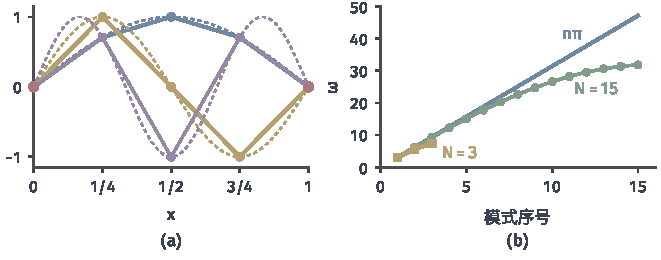
\includegraphics[width=112mm]{figures/06-differential-equations/02-partial-differential-equations/matplotlib/wave-discrete-modes/figure.pdf}
  \caption{珠链和连续弦的模式，$L=1$，$c=1$。(a)$N=3$时的三个特征向量（折线上的点），细虚线是连续模式$\sin(k\pi x)$，红点是固定端。(b)频率随模式序号的变化：蓝线是连续弦$n\pi$，绿线和黄线是$N=15$和$N=3$的珠链。}
  \label{fig:wave-discrete-modes}
\end{BookInlineFigure}


\section{受迫响应}
\label{sec:wave-forced}

弦上持续受力，或者端点被人摇动，解怎样由这些输入决定？线性问题的办法是把输入切成很多瞬时的小份，每一份单独算，再加起来。

\paragraph{脉冲等于初速度}
先看单个振子的例子。第~\ref{chap:linear-differential-systems}章的常数变易公式对$\ddot{x}+\omega^{2}x=g(t)$、零初值给出
\[
 x(t)=\int_0^{t}\frac{\sin\omega(t-s)}{\omega}\,g(s)\,\mathrm{d}s .
\]
被积函数中的$\sin\omega(t-s)/\omega$，是时刻$s$得到单位初速度之后，经过时间$t-s$的自由振动。外力在极短的时间$\mathrm{d}s$内提供的冲量是$g(s)\,\mathrm{d}s$，它的效果就是让速度突然增加这么多。

把振子换成弦，道理不变。时刻$s$的外力$f(\cdot,s)$在$\mathrm{d}s$内给弦增加的速度是$f(\cdot,s)\,\mathrm{d}s$，这相当于在时刻$s$从零位移出发，以这个速度分布开始一次自由振动。

\begin{theorem}[\term{Duhamel原理}（Duhamel's principle）]
\label{thm:wave-duhamel}
设$f$和$\partial_xf$在$\mathbb{R}\times[0,T]$上连续。对每个$s\in[0,T]$，记$w(\cdot,\cdot\,;s)$是自由波动方程在$t\geq s$上的解，它在时刻$s$的位移为零，速度为$f(\cdot,s)$。则
\begin{equation}
 u(x,t)=\int_0^{t}w(x,t;s)\,\mathrm{d}s=\frac1{2c}\int_0^{t}\int_{x-c(t-s)}^{x+c(t-s)}f(y,s)\,\mathrm{d}y\,\mathrm{d}s
 \label{eq:wave-duhamel}
\end{equation}
是$\partial_t^{2}u-c^{2}\partial_x^{2}u=f$在零初值下的$C^{2}$解。
\end{theorem}

\begin{proof}
由式~\eqref{eq:wave-dalembert}，从时刻$s$算起，$w$的表达式为
\[
 w(x,t;s)=\frac1{2c}\int_{x-c(t-s)}^{x+c(t-s)}f(y,s)\,\mathrm{d}y .
\]
它给出式~\eqref{eq:wave-duhamel}的第二个等号。直接求导，$\partial_tw$是$f$在两端点处值的平均，$\partial_t^{2}w$和$\partial_x^{2}w$都由$\partial_xf$在端点的值表示。这些导数对$(x,t,s)$连续，可以在积分号下求导。

对$t$求一次导，积分上限带来一项$w(x,t;t)$。这一项的积分区间长度为零，所以等于零：
\[
 \partial_tu(x,t)=w(x,t;t)+\int_0^{t}\partial_tw(x,t;s)\,\mathrm{d}s=\int_0^{t}\partial_tw(x,t;s)\,\mathrm{d}s .
\]

再求一次导，上限这次带来$\partial_tw(x,t;t)$，按定义它等于$f(x,t)$：
\[
 \partial_t^{2}u=f(x,t)+\int_0^{t}\partial_t^{2}w\,\mathrm{d}s=f(x,t)+c^{2}\int_0^{t}\partial_x^{2}w\,\mathrm{d}s=f+c^{2}\partial_x^{2}u .
\]
令$t=0$，由上面两式得$u(\cdot,0)=0$，$\partial_tu(\cdot,0)=0$。
\end{proof}

定理对$f$的光滑性要求来自$\partial_x^{2}w$要由$\partial_xf$表示。$f$只是连续甚至只是局部可积时，式~\eqref{eq:wave-duhamel}仍有意义，它给出的是弱解，下面持续施力的例子就属于这种情形。一般的初值问题由线性性得到：式~\eqref{eq:wave-dalembert}加上式~\eqref{eq:wave-duhamel}。

\paragraph{外力的依赖区域}
式~\eqref{eq:wave-duhamel}的积分区域是点$(x,t)$的回溯三角形，如图~\ref{fig:wave-duhamel}(a)。时刻$s$的外力只在宽度$2c(t-s)$的切片上起作用，越接近$t$，切片越窄。

三角形内的权重处处是常数$1/(2c)$。换个角度看图~\ref{fig:wave-duhamel}(b)：在点$(y,s)$施加单位脉冲，此后的响应在前向锥内是$1/(2c)$，锥外是零。这是实轴上的Green函数，用公式写是
\begin{equation}
 G(x,t;y,s)=\frac1{2c}\,\mathbb{I}\{\lvert x-y\rvert<c(t-s)\}.
 \label{eq:wave-green}
\end{equation}
式~\eqref{eq:wave-duhamel}就是用$G$对$f$积分。

\begin{BookInlineFigure}
  \centering
  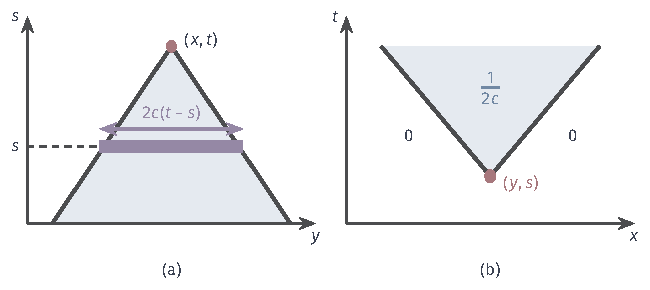
\includegraphics[width=110.06mm]{figures/06-differential-equations/02-partial-differential-equations/tikz/wave-duhamel/figure.pdf}
  \caption{外力的作用范围。(a)计算$u(x,t)$要积分回溯三角形内的$f$，紫色条带是时刻$s$的切片，宽度为$2c(t-s)$。(b)点$(y,s)$（红）的单位脉冲只在前向锥内产生响应，值为$1/(2c)$，锥外为零。}
  \label{fig:wave-duhamel}
\end{BookInlineFigure}

\paragraph{瞬时冲击与持续驱动}
比较两种施力方式，取$c=1$。一种是$t=0$时的一次单位冲击，相当于初速度$\mathbb{I}\{\lvert x\rvert<1\}$，第~\ref{sec:wave-dalembert}节已算出$u(0,t)=\min\{t,1\}$。另一种是在同一区间上持续施力，$f=\mathbb{I}\{\lvert x\rvert<1\}$对所有$t\geq0$成立。

持续驱动相当于每一时刻都敲一次。由式~\eqref{eq:wave-duhamel}，时刻$s$的那一次敲击到$t$时在$x=0$的贡献是$\min\{t-s,1\}$。令$r=t-s$，积分得到
\[
 u(0,t)=\int_0^{t}\min\{r,1\}\,\mathrm{d}r=
 \begin{cases}
  t^{2}/2, & 0\leq t\leq1,\\
  t-\frac12, & t\geq1.
 \end{cases}
\]

例如$t=1$时$u(0,1)=1/2$，$t=3$时$u(0,3)=5/2$。一次冲击的响应到$t=1$后不再变化；持续驱动的响应在$t>1$后线性增长，因为不断有新的敲击的贡献抵达这一点。

图~\ref{fig:wave-impulse-sustained}(a)显示持续驱动如何由各次冲击累加：浅色的梯形是时刻$s=2,1,0$的单次冲击到$t=3$时的响应，蓝色的钟形是所有时刻的积分。(b)是两种情形在原点处的时间历程。

\begin{BookInlineFigure}
  \centering
  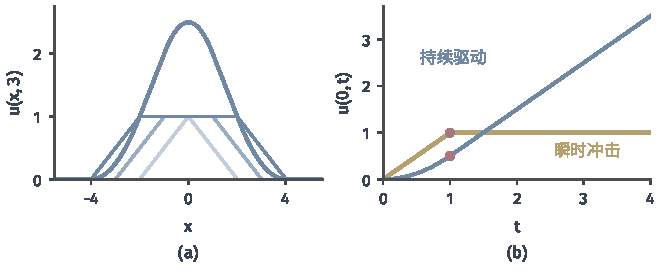
\includegraphics[width=112mm]{figures/06-differential-equations/02-partial-differential-equations/matplotlib/wave-impulse-sustained/figure.pdf}
  \caption{瞬时冲击与持续驱动，$c=1$，力作用在$(-1,1)$上。(a)$t=3$时的位移：蓝色由浅到深的三个梯形是时刻$s=2,1,0$的单次冲击的响应，粗蓝线是持续驱动的解，等于全部冲击响应的积分。(b)原点处的位移，黄线是一次冲击，蓝线是持续驱动，红点是$t=1$时的值$1$和$1/2$。}
  \label{fig:wave-impulse-sustained}
\end{BookInlineFigure}

\paragraph{有限区间：逐模式受迫与共振}
在$(0,L)$上两端固定，把解按式~\eqref{eq:wave-dirichlet-modes}的模式展开，每个系数$a_n(t)$都是一个受迫振子。设$f_n(t)$是$f(\cdot,t)$的正弦系数，零初值时
\begin{equation}
 \ddot{a}_n+\omega_n^{2}a_n=f_n(t),\qquad a_n(t)=\int_0^{t}\frac{\sin\omega_n(t-s)}{\omega_n}f_n(s)\,\mathrm{d}s .
 \label{eq:wave-modal-forcing}
\end{equation}

取$L=1$，$c=1$，$f=\sin(\pi x)\cos(\Omega t)$，只有第一个模式被驱动，固有频率是$\omega_1=\pi$。$\Omega\neq\pi$时，解是特解加上消去初值的齐次解：
\[
 a_1(t)=\frac{\cos\Omega t-\cos\pi t}{\pi^{2}-\Omega^{2}} .
\]
它一直有界。例如$\Omega=2$时，$\lvert a_1\rvert\leq2/(\pi^{2}-4)\approx0.34$。

当$\Omega=\pi$时，上式的分母为零。令$\Omega\to\pi$取极限，由L'Hôpital法则得到
\[
 a_1(t)=\frac{t\sin\pi t}{2\pi} .
\]
代入方程可以验证：$\ddot{a}_1=\cos\pi t-\pi^{2}a_1$。幅度随时间线性增长，这就是共振：外力每个周期都在弦运动的方向上推，能量持续积累。

对比热方程的同一模式。$\dot{a}+\pi^{2}a=\cos\pi t$的解是一个有界的振荡加上快速衰减的暂态，幅度约为$1/(\pi\sqrt{\pi^{2}+1})\approx0.096$。扩散会不断耗掉输入，所以没有共振。图~\ref{fig:wave-resonance}对比了这三种响应。

\begin{BookInlineFigure}
  \centering
  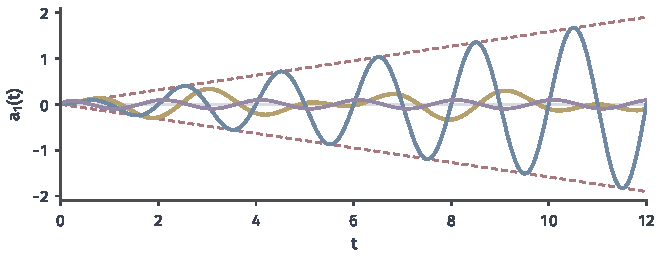
\includegraphics[width=112mm]{figures/06-differential-equations/02-partial-differential-equations/matplotlib/wave-resonance/figure.pdf}
  \caption{第一个模式在外力$\cos\Omega t$下的响应，$L=1$，$c=1$。蓝线是共振$\Omega=\pi$，红色虚线是它的包络$\pm t/(2\pi)$。黄线是非共振$\Omega=2$。紫线是热方程同一模式在$\Omega=\pi$下的响应。}
  \label{fig:wave-resonance}
\end{BookInlineFigure}

\paragraph{边界输入与能量}
除了体内的外力，也可以摇动端点。考虑半直线$x>0$，初值为零，左端按$u(0,t)=g(t)$运动，并设$g(0)=g'(0)=0$。此时右行波$u=g(t-x/c)$满足方程，并在$x=0$处取$g(t)$，所以解是
\begin{equation}
 u(x,t)=
 \begin{cases}
  g(t-x/c), & 0\leq x<ct,\\
  0, & x\geq ct .
 \end{cases}
 \label{eq:wave-boundary-solution}
\end{equation}
端点的运动沿特征线原样传到各处，只是延迟了$x/c$。

由式~\eqref{eq:wave-end-power}，端点的输入要算入能量账。这里$\partial_tu=g'$，$\partial_xu=-g'/c$，端点$x=0$的外法向导数是$-\partial_x$。把$\kappa$换成$c^{2}$（即除以线密度$\rho$），单位质量的输入功率是
\[
 P(t)=c^{2}\cdot\frac{g'(t)}{c}\cdot g'(t)=c\,g'(t)^{2}.
\]
弦原本静止时，摇动端点总在向弦输入能量，功率与端点速度的平方成正比，与$g$的符号无关。

取$c=1$，$g(t)=\sin^{2}\pi t$（$0\leq t\leq1$），此后$g=0$。这里$g'(t)=\pi\sin2\pi t$，$g''$在$t=0,1$有跳跃，所以解的二阶导数在两条特征线$x=t$和$x=t-1$上跳跃，其他位置方程按经典意义成立。累计输入的能量是
\[
 \int_0^{1}P(t)\,\mathrm{d}t=\int_0^{1}\pi^{2}\sin^{2}2\pi t\,\mathrm{d}t=\frac{\pi^{2}}2\approx4.93 .
\]

弦上的能量可以独立算一遍来核对。$t\geq1$时，由式~\eqref{eq:wave-boundary-solution}，$\partial_tu$和$\partial_xu$的平方都等于$g'(t-x)^{2}$，所以
\[
 E(t)=\frac12\int_0^{\infty}\bigl[(\partial_tu)^{2}+(\partial_xu)^{2}\bigr]\,\mathrm{d}x=\int_0^{1}g'(r)^{2}\,\mathrm{d}r=\frac{\pi^{2}}2 .
\]
两种算法结果相同，能量在端点停止摇动后保持不变，如图~\ref{fig:wave-boundary-drive}。

\begin{BookInlineFigure}
  \centering
  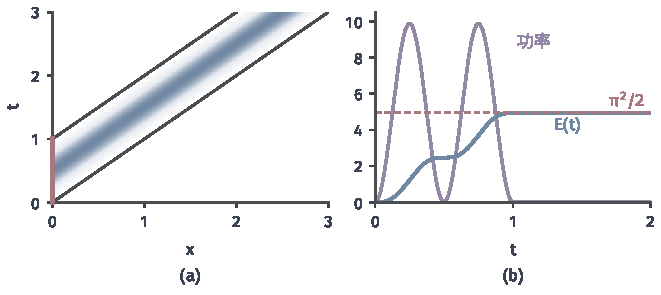
\includegraphics[width=112mm]{figures/06-differential-equations/02-partial-differential-equations/matplotlib/wave-boundary-drive/figure.pdf}
  \caption{端点驱动的半直线，$c=1$，$g(t)=\sin^{2}\pi t$（$0\leq t\leq1$，红色粗线）。(a)时空热图：端点的运动沿特征线传播，深灰直线是波包的前后沿。(b)输入功率$g'(t)^{2}$（紫）和弦上的能量$E(t)$（蓝，由空间积分算出），红色虚线是总输入$\pi^{2}/2$。}
  \label{fig:wave-boundary-drive}
\end{BookInlineFigure}

有限区间上，非齐次的边界条件可以转移成外力。若$u(0,t)=g(t)$，$u(L,t)=0$，令$R(x,t)=g(t)(1-x/L)$，$v=u-R$。$v$在两端为零，满足下面的方程，初值相应地减去$R$和$\partial_tR$在$t=0$的值：
\[
 \partial_t^{2}v-c^{2}\partial_x^{2}v=f-g''(t)\Bigl(1-\frac xL\Bigr).
\]
这样就回到了逐模式受迫的情形。此时端点的功率不一定为正，因为反射回来的波可以推动端点，把能量还给驱动源。


\section{能量估计}
\label{sec:wave-energy}

前面的计算反复出现同一个量：弦的动能加弹性能。不写出解，只对方程乘$\partial_tu$再积分，能得到什么？这样得到的结论不依赖一维公式，也不依赖模式展开，在一般区域上同样成立。

\paragraph{动能和弹性能}
线密度为$\rho$的弦，一小段的动能是$\frac12\rho(\partial_tu)^{2}\,\mathrm{d}x$。弹性能等于张力乘以伸长量，小斜率时一小段的伸长是$\sqrt{1+(\partial_xu)^{2}}\,\mathrm{d}x-\mathrm{d}x\approx\frac12(\partial_xu)^{2}\,\mathrm{d}x$，所以弹性能是$\frac12\kappa(\partial_xu)^{2}\,\mathrm{d}x$。除以$\rho$并推广到$\Omega\subset\mathbb{R}^{d}$，定义\term{动能}（kinetic energy）和\term{弹性能}（elastic energy）之和
\begin{equation}
 E(t)=\frac12\int_\Omega\bigl[(\partial_tu)^{2}+c^{2}\lVert\nabla u\rVert_2^{2}\bigr]\,\mathrm{d}\bm{x}.
 \label{eq:wave-energy}
\end{equation}

\begin{theorem}[能量恒等式]
\label{thm:wave-energy-identity}
设$\Omega\subset\mathbb{R}^{d}$有界，边界分片光滑，$u\in C^{2}(\overline{\Omega}\times[0,T])$满足$\partial_t^{2}u-c^{2}\Delta u=f$。则
\begin{equation}
 E'(t)=\int_\Omega f\,\partial_tu\,\mathrm{d}\bm{x}+c^{2}\int_{\partial\Omega}\partial_tu\,\partial_{\bm{n}}u\,\mathrm{d}S .
 \label{eq:wave-energy-identity}
\end{equation}
特别地，若$f\equiv0$，且边界每一处或者$\partial_tu=0$，或者$\partial_{\bm{n}}u=0$，则$E(t)$为常数。
\end{theorem}

\begin{proof}
积分号下对$t$求导，得到
\[
 E'(t)=\int_\Omega\bigl[\partial_tu\,\partial_t^{2}u+c^{2}\nabla u\cdot\nabla\partial_tu\bigr]\,\mathrm{d}\bm{x}.
\]

第二项用散度定理移走梯度，散度定理的条件和形式可参考\BookChapterRef{chap:integral-theorems}{卷二第27章“积分定理”}：
\[
 \int_\Omega\nabla u\cdot\nabla\partial_tu\,\mathrm{d}\bm{x}=\int_{\partial\Omega}\partial_tu\,\partial_{\bm{n}}u\,\mathrm{d}S-\int_\Omega\partial_tu\,\Delta u\,\mathrm{d}\bm{x}.
\]

代回去，体积分合并成$\int_\Omega\partial_tu(\partial_t^{2}u-c^{2}\Delta u)\,\mathrm{d}\bm{x}$，由方程等于$\int_\Omega f\partial_tu\,\mathrm{d}\bm{x}$。这就是式~\eqref{eq:wave-energy-identity}。无源且边界项为零时，$E'=0$。
\end{proof}

式~\eqref{eq:wave-energy-identity}是能量账：右端第一项是外力的功率，第二项是边界的功率，它正是式~\eqref{eq:wave-end-power}除以$\rho$。固定端、自由端以及给定不随时间变化的位移（此时$\partial_tu=0$）都不进出能量。

\paragraph{和热方程对比}
第~\ref{chap:diffusion-equations}章对热方程也做了能量估计，那里在同样的边界条件下乘的是$u$，得到的是
\[
 \frac{\mathrm{d}}{\mathrm{d}t}\,\frac12\int_\Omega u^{2}\,\mathrm{d}\bm{x}=-\int_\Omega\lVert\nabla u\rVert_2^{2}\,\mathrm{d}\bm{x}\leq0 .
\]
区别在于热方程的能量只含$u$，并且被梯度持续消耗；波动方程的能量同时含$\partial_tu$和$\nabla u$，两部分互相转换，总量不变。这也和两个方程的时间方向性相合：波动方程把$t$换成$-t$仍是波动方程，能量守恒在两个时间方向都成立；热方程只能向前。

\paragraph{手算一个能量账}
继续用中点拨起的弦，$L=1$，$c=1$。$t=0$时速度为零，$\lvert u_0'\rvert=1$几乎处处成立，所以由式~\eqref{eq:wave-energy}，
\[
 E(0)=\frac12\int_0^{1}1\,\mathrm{d}x=\frac12 .
\]

能量也可以按模式计算。把式~\eqref{eq:wave-series}代入式~\eqref{eq:wave-energy}，由三角函数的正交性，不同模式的交叉项为零，每个模式的能量单独守恒：
\begin{equation}
 E=\frac L4\sum_{n=1}^{\infty}\bigl(\omega_n^{2}a_n^{2}+b_n^{2}\bigr).
 \label{eq:wave-modal-energy}
\end{equation}

代入式~\eqref{eq:wave-pluck-coefficients}。只有奇数$n$的项非零，$\omega_n^{2}a_n^{2}=16/(n^{2}\pi^{2})$，于是
\[
 E=\frac14\sum_{n\ \text{奇}}\frac{16}{n^{2}\pi^{2}}=\frac4{\pi^{2}}\sum_{n\ \text{奇}}\frac1{n^{2}}=\frac4{\pi^{2}}\cdot\frac{\pi^{2}}8=\frac12 .
\]
两种算法一致。这里折线初值只是分段光滑，定理~\ref{thm:wave-energy-identity}不能直接用，但式~\eqref{eq:wave-modal-energy}对$H_0^{1}\times L^{2}$的数据仍然成立。第一项占$4/\pi^{2}\approx0.405$，即总能量的$81\%$；加上$n=3$后达$90\%$，加上$n=5$后达$93\%$。高频模式的系数虽小，乘上$\omega_n^{2}$后对能量的贡献并不小。

\paragraph{能量守恒不等于振幅不变}
能量不变，弦上各点的位移却可以大幅变化。回到实轴上的帐篷形初值，由式~\eqref{eq:wave-tent-solution}，$t=0$时能量全是弹性能：
\[
 E=\frac12\int_{-1}^{1}1\,\mathrm{d}x=1,\qquad \max_{x}\lvert u(x,0)\rvert=1.
\]

$t\geq1$时分成两列互不重叠的波，每列的$\partial_tu$和$\partial_xu$的平方都是$1/4$，在长度为$2$的支集上，动能和弹性能都是$\frac12\cdot\frac14\cdot2$，两列相加得到
\[
 K=\frac12,\qquad V=\frac12,\qquad \max_{x}\lvert u(x,t)\rvert=\frac12.
\]
最大位移减半，总能量不变，只是一半的弹性能变成了动能。

图~\ref{fig:wave-energy-accounting}对比了这几种情形。(a)是拨弦的动能和弹性能相互转换，总和恒为$1/2$。(b)是同一初值下热方程的$\frac12\lVert u\rVert_2^{2}$，单调衰减。(c)是实轴上的帐篷，总能量不变，最大位移却下降。

\begin{BookInlineFigure}
  \centering
  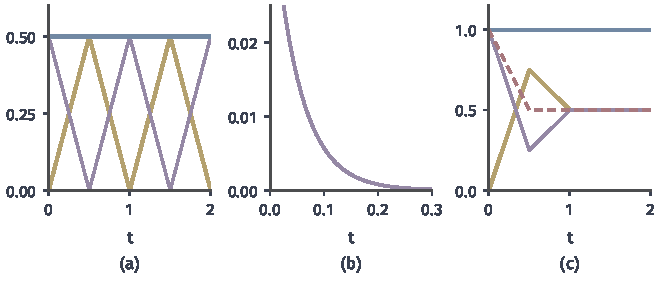
\includegraphics[width=112mm]{figures/06-differential-equations/02-partial-differential-equations/matplotlib/wave-energy-accounting/figure.pdf}
  \caption{能量账。(a)拨弦，$L=1$，$c=1$：黄线是动能，紫线是弹性能，蓝线是两者之和。(b)同一初值在热方程下的$\frac12\lVert u\rVert_2^{2}$（紫），单调下降。(c)实轴上的帐篷：黄、紫、蓝含义同(a)，红色虚线是最大位移，从$1$降到$1/2$，能量却保持为$1$。}
  \label{fig:wave-energy-accounting}
\end{BookInlineFigure}

\paragraph{差解的能量给出唯一性}
能量恒等式最直接的用途是唯一性：设两个解有相同的数据，它们的差的能量从零开始，又不会增加。

\begin{theorem}[唯一性]
\label{thm:wave-uniqueness}
设$\Omega$有界，边界分片光滑。式~\eqref{eq:wave-ibvp}在每一处边界上指定$u$或$\partial_{\bm{n}}u$的条件下，至多有一个$C^{2}(\overline{\Omega}\times[0,T])$解。
\end{theorem}

\begin{proof}
设$u,\tilde{u}$是两个解，$w=u-\tilde{u}$。由线性性，$w$满足无源方程、零初值和齐次的边界条件：在指定$u$的边界上$w=0$，从而$\partial_tw=0$；在指定$\partial_{\bm{n}}u$的边界上$\partial_{\bm{n}}w=0$。定理~\ref{thm:wave-energy-identity}给出$w$的能量为常数，而零初值使它在$t=0$时为零，所以
\[
 \int_\Omega\bigl[(\partial_tw)^{2}+c^{2}\lVert\nabla w\rVert_2^{2}\bigr]\,\mathrm{d}\bm{x}=0,\qquad 0\leq t\leq T.
\]

被积函数连续且非负，所以处处为零，特别地$\partial_tw\equiv0$。于是$w(\bm{x},t)=w(\bm{x},0)=0$。
\end{proof}

边界条件在这里是必需的。在$(0,1)$上取$c=1$，零初值，如果不给边界条件，$u\equiv0$是解，而式~\eqref{eq:wave-boundary-solution}的右行波$g(t-x)$（$g$在$t$很小时为零）也是解：它们的初值相同，差别只来自左端的输入。边界条件正是用来堵住这种能量入口的。

这个证明没有用到解的公式。第~\ref{sec:wave-modes}节的级数解的唯一性由此得到。同样的思路用于有限时间的连续依赖，见下面的增长估计。

\paragraph{外力下的能量增长}
含源项时能量不再守恒，但能估计它增长多快。由式~\eqref{eq:wave-energy-identity}，边界项为零时，Cauchy--Schwarz不等式给出
\[
 E'(t)\leq\lVert f(\cdot,t)\rVert_{L^{2}(\Omega)}\,\lVert\partial_tu(\cdot,t)\rVert_{L^{2}(\Omega)} .
\]

动能不超过总能量，所以$\lVert\partial_tu\rVert_{L^{2}}\leq\sqrt{2E}$，从而
\[
 E'(t)\leq\sqrt2\,\lVert f(\cdot,t)\rVert_{L^{2}(\Omega)}\sqrt{E(t)} .
\]

这种形式的不等式适合对$\sqrt{E}$积分。为了避免$E=0$时除以零，先对$\varepsilon>0$考虑$\sqrt{E+\varepsilon}$，求导后代入上式，得到
\[
 \frac{\mathrm{d}}{\mathrm{d}t}\sqrt{E+\varepsilon}=\frac{E'}{2\sqrt{E+\varepsilon}}\leq\frac1{\sqrt2}\lVert f(\cdot,t)\rVert_{L^{2}(\Omega)} .
\]
积分后令$\varepsilon\to0$，就得到下面的定理。

\begin{theorem}[能量增长估计]
\label{thm:wave-energy-growth}
在定理~\ref{thm:wave-energy-identity}的条件下，设边界项为零。则对$0\leq t\leq T$，
\begin{equation}
 \sqrt{E(t)}\leq\sqrt{E(0)}+\frac1{\sqrt2}\int_0^{t}\lVert f(\cdot,s)\rVert_{L^{2}(\Omega)}\,\mathrm{d}s .
 \label{eq:wave-energy-growth}
\end{equation}
\end{theorem}

用在两组数据的差解上，式~\eqref{eq:wave-energy-growth}给出有限时间内对$(u_0,u_1,f)$的连续依赖，度量是能量范数。

这个估计的增长速度和共振是相合的。继续第~\ref{sec:wave-forced}节的例子，$L=1$，$c=1$，$f=\sin(\pi x)\cos\pi t$。外力的范数和能量分别是
\[
 \lVert f(\cdot,t)\rVert_{L^{2}}=\frac{\lvert\cos\pi t\rvert}{\sqrt2},\qquad E(t)=\frac14\bigl(\dot{a}_1^{2}+\pi^{2}a_1^{2}\bigr),
\]
后者由式~\eqref{eq:wave-modal-energy}对时变系数的同样计算得到。

在$t=12$处，由$a_1=t\sin\pi t/(2\pi)$得$a_1(12)=0$，$\dot{a}_1(12)=6$，所以$\sqrt{E(12)}=3$。式~\eqref{eq:wave-energy-growth}的右端是
\[
 \frac12\int_0^{12}\lvert\cos\pi s\rvert\,\mathrm{d}s=\frac12\cdot12\cdot\frac2\pi=\frac{12}{\pi}\approx3.82 .
\]
上界成立，两者都随$t$线性增长，估计的阶是准确的。如图~\ref{fig:wave-energy-growth}，非共振的$\Omega=2$只让能量有界振荡，这时上界就偏松了：式~\eqref{eq:wave-energy-growth}只用到$\lVert f\rVert_{L^{2}}$，看不到外力和模式频率是否匹配。

\begin{BookInlineFigure}
  \centering
  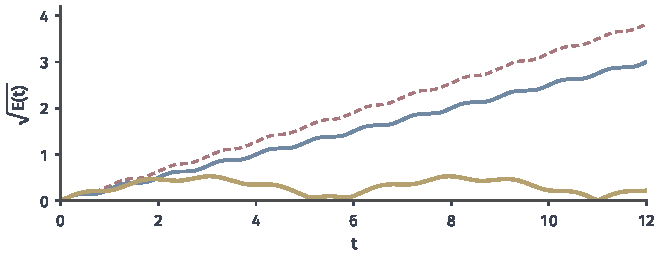
\includegraphics[width=112mm]{figures/06-differential-equations/02-partial-differential-equations/matplotlib/wave-energy-growth/figure.pdf}
  \caption{外力下的$\sqrt{E(t)}$，$L=1$，$c=1$，零初值，$f=\sin(\pi x)\cos\Omega t$。蓝线是共振$\Omega=\pi$，红色虚线是它的上界~\eqref{eq:wave-energy-growth}，两者都线性增长。黄线是非共振$\Omega=2$，能量有界。}
  \label{fig:wave-energy-growth}
\end{BookInlineFigure}


\section{有限传播}
\label{sec:wave-finite-speed}

一维公式告诉我们扰动以速度$c$传播。公式本身不能搬到高维，但这个结论能否脱离公式、在任意维成立？答案是能，用的是把能量局部化到一个收缩的球上。

\paragraph{收缩球上的能量}
设$u$在$\mathbb{R}^{d}$上解无源波动方程。取一点$(\bm{x}_0,t_0)$，考虑以$\bm{x}_0$为中心、半径随时间减小的球：
\[
 B_t=B\bigl(\bm{x}_0,\,c(t_0-t)\bigr),\qquad 0\leq t<t_0 .
\]
这些球叠起来就是顶点在$(\bm{x}_0,t_0)$的\term{传播锥}（propagation cone），如图~\ref{fig:wave-cone-proof}：
\begin{equation}
 K=\bigl\{(\bm{x},t):\lVert\bm{x}-\bm{x}_0\rVert_2\leq c(t_0-t),\ 0\leq t\leq t_0\bigr\}.
 \label{eq:wave-cone}
\end{equation}

直观上，球内的能量有两种变化。一是通过球面的能量通量，它可能把能量带进来；二是球在缩小，边缘上的能量被甩到球外。下面的计算说明，后者足以抵消前者，这恰好需要收缩的速度等于波速。

\begin{BookInlineFigure}
  \centering
  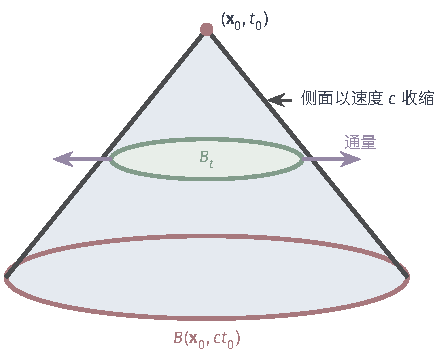
\includegraphics[width=75.406mm]{figures/06-differential-equations/02-partial-differential-equations/tikz/wave-cone-proof/figure.pdf}
  \caption{传播锥。绿色圆盘是时刻$t$的球$B_t$，红色边界是初始的球$B(\bm{x}_0,ct_0)$。紫色箭头是通过球面的能量通量，球的半径以速度$c$减小，通量带来的增量被缩小带走的能量抵消。}
  \label{fig:wave-cone-proof}
\end{BookInlineFigure}

\begin{theorem}[\term{有限传播速度}（finite speed of propagation）]
\label{thm:wave-finite-speed}
设$u\in C^{2}(\mathbb{R}^{d}\times[0,T])$满足$\partial_t^{2}u=c^{2}\Delta u$，$0<t_0\leq T$。若在球$B(\bm{x}_0,ct_0)$上$u_0=u_1=0$，则在传播锥$K$上$u=0$。
\end{theorem}

\begin{proof}
定义局部能量
\[
 e(t)=\frac12\int_{B_t}\bigl[(\partial_tu)^{2}+c^{2}\lVert\nabla u\rVert_2^{2}\bigr]\,\mathrm{d}\bm{x},\qquad 0\leq t<t_0 .
\]
半径变化的球上的积分对$t$求导，除了被积函数的导数，还要加上半径的变化率乘以球面上的积分，这里半径变化率是$-c$。于是
\[
 e'(t)=\int_{B_t}\bigl[\partial_tu\,\partial_t^{2}u+c^{2}\nabla u\cdot\nabla\partial_tu\bigr]\,\mathrm{d}\bm{x}-\frac c2\int_{\partial B_t}\bigl[(\partial_tu)^{2}+c^{2}\lVert\nabla u\rVert_2^{2}\bigr]\,\mathrm{d}S .
\]

和定理~\ref{thm:wave-energy-identity}的证明一样，第一个积分用散度定理和方程化成球面积分，$\bm{n}$为球面的外法向：
\[
 e'(t)=\int_{\partial B_t}\Bigl[c^{2}\partial_tu\,\partial_{\bm{n}}u-\frac c2(\partial_tu)^{2}-\frac{c^{3}}2\lVert\nabla u\rVert_2^{2}\Bigr]\,\mathrm{d}S .
\]

现在估计第一项。法向导数是梯度在单位向量上的分量，所以它的绝对值不超过梯度的范数：
\[
 \lvert\partial_{\bm{n}}u\rvert\leq\lVert\nabla u\rVert_2 .
\]
再对$\lvert\partial_tu\rvert$和$c\lVert\nabla u\rVert_2$用均值不等式：
\[
 c^{2}\lvert\partial_tu\rvert\,\lvert\partial_{\bm{n}}u\rvert\leq c\cdot\lvert\partial_tu\rvert\cdot c\lVert\nabla u\rVert_2\leq\frac c2(\partial_tu)^{2}+\frac{c^{3}}2\lVert\nabla u\rVert_2^{2} .
\]
被积函数因此不超过零，$e'(t)\leq0$。

由假设$e(0)=0$，而$e\geq0$，所以$e(t)=0$对$0\leq t<t_0$成立。于是在$K$内$\partial_tu=0$且$\nabla u=0$。对$K$内任一点$(\bm{x},t)$，线段$\{(\bm{x},s):0\leq s\leq t\}$都在$K$内，沿它积分得$u(\bm{x},t)=u(\bm{x},0)=0$。
\end{proof}

证明中均值不等式的系数恰好是$c/2$，这说明波速$c$是能用的最小收缩速度。球若以更慢的速度收缩，结论就不再成立。取$d=1$，$c=1$，向右传播的帐篷$u=\Lambda(x+5-t)$，支集在$[t-6,t-4]$。$t=0$时支集是$[-6,-4]$，所以$u_0,u_1$在$(-4,4)$上都为零。

让半径按$R(t)=4-t/2$缩小，速度只有$1/2$。这个慢收缩的区间的左端$-R(t)$向右移动得比波包慢，波包追上并进入区间：$t=0$时局部能量为$0$，$t=4$时波包全部在$[-2,0]$内，局部能量等于波包的全部能量$2$。特别地，$u(0,5)=\Lambda(0)=1\neq0$。但这并不违反定理：以$B(0,4)$为底、以速度$1$收缩的锥顶点在$t=4$，点$(0,5)$在锥外。

证明只用到$K$内的方程，所以源项在$K$内为零时结论仍然成立。在有界区域上，只要传播锥不碰到边界，结论就不变；锥碰到固定端或自由端时，边界上的通量项为零，同样的估计在球与$\Omega$的交上仍然有效，端点的影响体现为反射，传播速度依然不超过$c$。

\paragraph{用帐篷核对局部能量}
取$d=1$，$c=1$，帐篷初值，$(x_0,t_0)=(0,3)$，锥在时刻$t$的截面是$\lvert x\rvert\leq3-t$。解$u=F(x-t)+G(x+t)$时，
\[
 (\partial_tu)^{2}+(\partial_xu)^{2}=2F'(x-t)^{2}+2G'(x+t)^{2},
\]
交叉项相消。这里$F=G=\frac12\Lambda$，$\lvert F'\rvert=\frac12$，所以每列波在支集上的能量密度是$\frac12\cdot2\cdot\frac14=\frac14$，长度为$2$，每列带能量$1/2$。

右行波的支集是$[t-1,t+1]$。$t\leq1$时它全在截面内，$e(t)=1$。$t\geq2$时$t-1\geq3-t$，它全部离开截面，$e(t)=0$。$1<t<2$时，留在截面内的长度是$(3-t)-(t-1)=4-2t$，左右两列对称，于是
\begin{equation}
 e(t)=2\cdot\frac14\cdot(4-2t)=2-t,\qquad 1\leq t\leq2.
 \label{eq:wave-local-energy-example}
\end{equation}

这条曲线画在图~\ref{fig:wave-cone-energy}(b)中。局部能量从不增加，波包穿过锥面时能量离开，这正是定理证明中的不等式。(a)是同一过程的时空图。

\begin{BookInlineFigure}
  \centering
  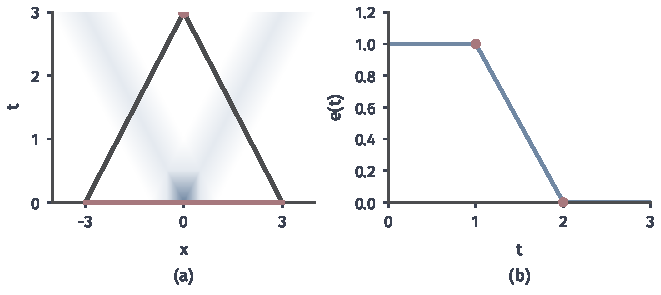
\includegraphics[width=112mm]{figures/06-differential-equations/02-partial-differential-equations/matplotlib/wave-cone-energy/figure.pdf}
  \caption{帐篷解的局部能量，$c=1$，$(x_0,t_0)=(0,3)$。(a)时空图，深灰三角形是传播锥，红色线段是底面。两个波包在$1<t<2$时穿出锥面。(b)由数值积分算出的$e(t)$（蓝），红点标出$t=1,2$，中间一段是式~\eqref{eq:wave-local-energy-example}的直线。}
  \label{fig:wave-cone-energy}
\end{BookInlineFigure}

\paragraph{依赖区域与影响区域}
定理~\ref{thm:wave-finite-speed}可以换一种说法。对线性问题，两个解之差仍是解，所以定理说明：两组初值若在$B(\bm{x}_0,ct_0)$上相同，解在点$(\bm{x}_0,t_0)$的值也相同。这引出下面两个概念。

\begin{definition}[依赖区域与影响区域]
\label{def:wave-domains}
点$(\bm{x}_0,t_0)$的\term{依赖区域}（domain of dependence）是初始时刻的闭球$\overline{B}(\bm{x}_0,ct_0)$。集合$A\subset\mathbb{R}^{d}$的\term{影响区域}（domain of influence）是
\begin{equation}
 \bigl\{(\bm{x},t):t\geq0,\ \mathrm{dist}(\bm{x},A)\leq ct\bigr\}.
 \label{eq:wave-influence}
\end{equation}
\end{definition}

由定理~\ref{thm:wave-finite-speed}，若$u_0,u_1$的支集在$A$内，则$\mathrm{dist}(\bm{x},A)>ct$时$u(\bm{x},t)=0$：以$\bm{x}$为中心、$ct$为半径的球与$A$不相交，初值在球上为零。一维时这两个区域就是图~\ref{fig:wave-dependence}。

定义给出的是“最多”依赖哪些数据，真正依赖的集合可能更小。一维时初始位移只用到两个端点，定理~\ref{thm:wave-finite-speed}无法看出这一点，它只说依赖不会超出球。

\paragraph{与热方程比较}
热方程的解由热核表示。第~\ref{chap:diffusion-equations}章的热核在一维是下面的Gauss函数，$\partial_tu=\partial_x^{2}u$的解是它与初值的卷积：
\[
 \Phi(x,t)=\frac1{\sqrt{4\pi t}}\exp\Bigl(-\frac{x^{2}}{4t}\Bigr),\qquad t>0 .
\]
$\Phi$处处为正，所以非负且不恒为零的初值在任何正时刻都使解处处为正。扰动的“速度”是无穷大的，这和有限传播形成对比。

这个差别需要谨慎理解。取$x=2$，$t=0.01$，单位点源的热核值是
\[
 \Phi(2,0.01)=\frac{\mathrm{e}^{-100}}{\sqrt{0.04\pi}}\approx1.0\times10^{-43},
\]
严格为正，但实际上探测不到。热方程的“无穷速度”是数学结论，物理上是极微弱的尾部。波动方程的前沿外严格为零，不存在尾部。图~\ref{fig:wave-vs-heat-spread}在同一帐篷初值下比较了两者，(c)取对数坐标才看得到热方程的尾部。

\begin{BookInlineFigure}
  \centering
  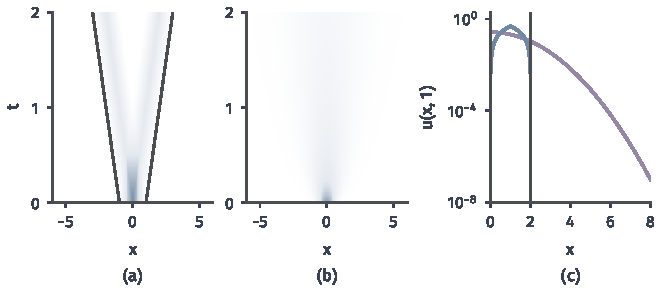
\includegraphics[width=112mm]{figures/06-differential-equations/02-partial-differential-equations/matplotlib/wave-vs-heat-spread/figure.pdf}
  \caption{同一帐篷初值的传播。(a)波动方程（$c=1$）的时空图，深灰线是传播前沿，线外严格为零。(b)热方程（扩散系数为$1$）的时空图，无明确前沿，鼓包逐渐抹平。(c)$t=1$时的对数坐标：紫线是热方程的解，始终为正；蓝线是波动方程的解，到深灰竖线$x=2$处截止。}
  \label{fig:wave-vs-heat-spread}
\end{BookInlineFigure}

\paragraph{耗散与平滑}
除了传播范围，两个方程在耗散和平滑上的差别也来自时间因子。由式~\eqref{eq:wave-pluck-coefficients}，拨弦的第$9$个系数是$a_9=4/(81\pi^{2})\approx0.0050$。$t=0.1$时，$L=1$的两种时间因子分别是
\[
 \mathrm{e}^{-81\pi^{2}\cdot0.1}\approx1.9\times10^{-35},\qquad \cos(0.9\pi)\approx-0.95 .
\]

热方程几乎抹掉了这个模式，波动方程只是改变了它的符号。把所有高频模式放在一起，热方程的解在任意正时刻都是光滑的，波动方程的折角却原样保留，因此逐点的光滑性不可能改善。

反过来，波动方程也没有扩散方程那样的不可逆性。能量不耗散，时间反向后问题仍然适定，高频成分不会在反向时被放大。第~\ref{chap:diffusion-equations}章的逆热问题之所以不稳定，正是因为反向时需要除以极小的因子$\mathrm{e}^{-n^{2}\pi^{2}t}$，而这里的因子模长始终不超过$1$，没有小到需要除的问题。

\paragraph{不要把一维公式搬到高维}
d'Alembert公式依赖换元~\eqref{eq:wave-characteristic-form}，而高维方向不止左右两个，公式没有直接的推广。三维的径向解可以说明这一点。对只依赖$r=\lVert\bm{x}\rVert_2$的函数，$\Delta u=r^{-1}\partial_r^{2}(ru)$，所以$ru$满足一维波动方程。取支集在$(a,b)$内（$a>0$）的光滑函数$\varphi$，外传的球面波是
\begin{equation}
 u(\bm{x},t)=\frac{\varphi(r-ct)}{r} .
 \label{eq:wave-spherical}
\end{equation}
它的幅度按$1/r$衰减，而能量由定理~\ref{thm:wave-energy-identity}（用足够大的球）保持不变：能量摊到越来越大的球面上，每点的振幅自然下降。这比一维行波多了一个衰减因子，是能量守恒与振幅不变并非一回事的另一个例子。

点脉冲的响应在不同维数中的差别更大，如图~\ref{fig:wave-point-response-dimensions}（$c=1$，$t=1$）。一维的响应是$(-1,1)$上的常数$1/2$，前沿过后留下平台。二维的响应在圆盘内是$1/(2\pi\sqrt{1-r^{2}})$，前沿过后留有逐渐衰减的尾巴。三维的响应集中在球面$r=1$上，前沿过后立即归零。这些公式的推导要用到球面平均和降维，篇幅较长，读者可查阅偏微分方程教材。这里要记住的是：前沿之外为零在所有维数中都成立，这是定理~\ref{thm:wave-finite-speed}保证的；前沿之内的形状随维数变化，不能由一维类推。

\begin{BookInlineFigure}
  \centering
  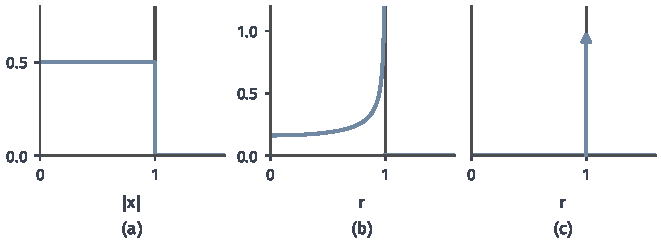
\includegraphics[width=112mm]{figures/06-differential-equations/02-partial-differential-equations/matplotlib/wave-point-response-dimensions/figure.pdf}
  \caption{原点处单位脉冲在$t=1$的响应，$c=1$，横轴为到原点的距离。(a)一维：前沿内是常数$1/2$。(b)二维：前沿内是$1/(2\pi\sqrt{1-r^{2}})$，在$r=1$处发散。(c)三维：全部集中在球面$r=1$上（箭头表示$\delta$分布）。深灰竖线是前沿$r=1$，三种情形在前沿外都为零。}
  \label{fig:wave-point-response-dimensions}
\end{BookInlineFigure}


\section{本章小结}
\label{sec:wave-summary}

本章是椭圆方程和扩散方程之后的补充，讨论二阶时间演化的基本认识。由弦的受力得到波动方程，弯曲决定加速度，所以初始状态是位移和速度一对函数。

一维实轴上，d'Alembert公式把解写成一列右行波和一列左行波。初始位移分成两半走开，初始速度留下不断变宽的平台，依赖区域由两条特征线截出。端点通过反射起作用：固定端翻转，自由端不翻转。

区间上的解按边界条件允许的模式展开，时间因子是不衰减的简谐振动，驻波正是两列行波的叠加。外力用Duhamel原理化成脉冲的叠加，模式频率与外力匹配时出现共振，边界驱动也按功率进入能量账。

表~\ref{tab:wave-summary}对比了扩散方程和波动方程。

\begin{BookInlineTable}
  \centering
  \caption{扩散方程与波动方程的对比}
  \label{tab:wave-summary}
  \begin{tabular}{lll}
    \toprule
    & 扩散方程 & 波动方程\\
    \midrule
    时间阶数 & 一阶 & 二阶\\
    初值 & $u_0$ & $u_0,u_1$\\
    模式因子 & 指数衰减 & 简谐振荡\\
    能量 & $\frac12\lVert u\rVert_2^{2}$单调减小 & 动能加弹性能守恒\\
    传播速度 & 无穷（尾部极弱） & 不超过$c$\\
    折角 & 立即消失 & 沿特征线传播\\
    时间反向 & 不适定 & 适定\\
    外力下 & 无共振 & 共振时线性增长\\
    \bottomrule
  \end{tabular}
\end{BookInlineTable}

能量恒等式不依赖解的公式，由它得到守恒、唯一性和有限时间的增长估计；局部能量进一步给出有限传播速度，在任意维成立。能量守恒不等于振幅不变，前沿之外为零也不说明前沿之内的形状相同，这两点要与一维公式分开理解。

本章只讨论常系数的标量波动方程和有限时间的结论。变系数介质、弹性力学和电磁学中的波动系统，要在具体物理建模需要时，再按一般的双曲系统扩展。

